%%%%%%%%%%%%%%%%%%%%%%%%%%%%%%%%%%%%%%%%%
% Masters/Doctoral Thesis 
% LaTeX Template
%
% This template was downloaded from:
% http://www.LaTeXTemplates.com
%
% Version 2.x major modifications by:
% Vel (vel@latextemplates.com)
%
% Original Authors:
% Vel (vel@latextemplates.com)
% Johannes Böttcher
% Steve Gunn (http://users.ecs.soton.ac.uk/srg/softwaretools/document/templates/)
% Sunil Patel (http://www.sunilpatel.co.uk/thesis-template/)
%
% This template was modified by Muneendra Ojha to suit the needs of 
% IIIT Allahabad Students. This is a basic template consisting of all 
% requirements as approved by the institute. Please feel free to contact
% if any errors are found or updates needed.
% 
% Do not remove this preamble. Always remember to give credits where it is due.
% 
% Template license:
% CC BY-NC-SA 3.0 (http://creativecommons.org/licenses/by-nc-sa/3.0/)
%
%%%%%%%%%%%%%%%%%%%%%%%%%%%%%%%%%%%%%%%%%

%----------------------------------------------------------------------------------------
%	PACKAGES AND OTHER DOCUMENT CONFIGURATIONS
%----------------------------------------------------------------------------------------

\documentclass[
12pt, % The default document font size, options: 10pt, 11pt, 12pt
oneside, % Two side (alternating margins) for binding by default, uncomment to switch to one side
english, % ngerman for German
singlespacing, % options: singlespacing, onehalfspacing or doublespacing
%draft, % Uncomment to enable draft mode (no pictures, no links, overfull hboxes indicated)
% nolistspacing, % If the document is onehalfspacing or doublespacing, uncomment this to set spacing in lists to single
liststotoc, % Uncomment to add the list of figures/tables/etc to the table of contents
% toctotoc, % Uncomment to add the main table of contents to the table of contents
parskip, % Uncomment to add space between paragraphs
%nohyperref, % Uncomment to not load the hyperref package
headsepline, % Uncomment to get a line under the header
% chapterinoneline, % Uncomment to place the chapter title next to the number on one line
% consistentlayout, % Uncomment to change the layout of the declaration, abstract and acknowledgements pages to match the default layout
]{Thesis} % The class file specifying the document structure



\usepackage[utf8]{inputenc} % Required for inputting international characters
\usepackage[T1]{fontenc} % Output font encoding for international characters
\usepackage{lmodern} % Use modern standard font to prevent T1/scsl fallback warnings
\usepackage[backend=biber,
style=numeric,
bibencoding=utf8,
% style=authoryear, % if using style as authoryear, then cite the reference using \parencite{}
% style=reading
]{biblatex}
\addbibresource{example.bib} % The filename of the bibliography
\usepackage[autostyle=true]{csquotes} % Required to generate language-dependent quotes in the bibliography
\usepackage{array}% http://ctan.org/pkg/array
\usepackage{lipsum}
\usepackage{tikz} % For drawing diagrams natively
\usetikzlibrary{shapes.geometric, arrows.meta, positioning, fit, calc}
\usepackage{tabularx} % For responsive tables
\usepackage{booktabs} % For professional table rules
\usepackage{listings} % For code snippets in appendix
\usepackage{xcolor} % For coloring code snippets

\lstset{
  basicstyle=\ttfamily\footnotesize,
  backgroundcolor=\color{gray!5},
  frame=single,
  breaklines=true,
  keywordstyle=\color{blue},
  commentstyle=\color{green!50!black},
  stringstyle=\color{red},
  showstringspaces=false
}



%----------------------------------------------------------------------------------------
%	MARGIN SETTINGS
%----------------------------------------------------------------------------------------

\geometry{
	paper=a4paper, % Change to letterpaper for US letter
	inner=20mm, % Inner margin
	outer=20mm, % Outer margin
	bindingoffset=5mm, % Binding offset
	top=25mm, % Top margin
	bottom=20mm, % Bottom margin
	%showframe, % Uncomment to show how the type block is set on the page
}


%----------------------------------------------------------------------------------------
%	★★★ FILL IN YOUR INFORMATION HERE ★★★
%   THIS IS THE ONLY SECTION YOU NEED TO EDIT!
%----------------------------------------------------------------------------------------

% ============================================================
% THESIS DETAILS
% ============================================================
\thesistitle{IIITA Timetabling System}
\degree{Bachelor of Technology}  % Options: Bachelor of Technology, Master of Technology, Doctor of Philosophy

% ============================================================
% SUPERVISOR DETAILS
% ============================================================
\supervisor{Dr. Gaurav Srivastava}

% ============================================================
% STUDENT 1 DETAILS (Required - at least one student)
% ============================================================
\newcommand{\studentonename}{Eshant}
\newcommand{\studentoneroll}{IIT2023198}

% ============================================================
% STUDENT 2 DETAILS (Optional - comment out if only 1 student)
% ============================================================
\newcommand{\studenttwoname}{Rahul Roy}
\newcommand{\studenttworoll}{IIT2023196}

% ============================================================
% STUDENT 3 DETAILS (Optional - comment out if only 2 students)
% ============================================================
\newcommand{\studentthreename}{Lakavath Peer Singh}
\newcommand{\studentthreeroll}{IIT2023197}

% ============================================================
% DEPARTMENT & UNIVERSITY (Usually don't need to change)
% ============================================================
\department{Department of Information Technology}
\university{Indian Institute of Information Technology, Allahabad}
\subject{Information Technology}

% ============================================================
% HELPER COMMANDS - DO NOT EDIT BELOW THIS LINE
% These automatically format the student information
% ============================================================

% Format for title page (with line breaks)
\newcommand{\studentnamesformatted}{%
\studentonename%
\ifdefined\studenttwoname%
\\\studenttwoname%
\fi%
\ifdefined\studentthreename%
\\\studentthreename%
\fi%
}

\newcommand{\rollnumbersformatted}{%
\studentoneroll%
\ifdefined\studenttworoll%
\\\studenttworoll%
\fi%
\ifdefined\studentthreeroll%
\\\studentthreeroll%
\fi%
}

% Format for certificate (comma separated)
\newcommand{\studentnamescomma}{%
\studentonename%
\ifdefined\studenttwoname%
, \studenttwoname%
\fi%
\ifdefined\studentthreename%
, \studentthreename%
\fi%
}

% Format for declaration (with roll numbers)
\newcommand{\studentnamesdeclaration}{%
\studentonename{} (\studentoneroll)%
\ifdefined\studenttwoname%
, \studenttwoname{} (\studenttworoll)%
\fi%
\ifdefined\studentthreename%
, and \studentthreename{} (\studentthreeroll)%
\fi%
}

% Format for signatures
\newcommand{\studentsignatures}{%
\studentonename{} (\studentoneroll)%
\ifdefined\studenttwoname%
\\\studenttwoname{} (\studenttworoll)%
\fi%
\ifdefined\studentthreename%
\\\studentthreename{} (\studentthreeroll)%
\fi%
}

% Pronoun selection (I/We)
\newcommand{\pronounwe}{%
\ifdefined\studenttwoname%
We%
\else%
I%
\fi%
}

\newcommand{\pronounour}{%
\ifdefined\studenttwoname%
our%
\else%
my%
\fi%
}

% Legacy compatibility
\firstauthor{\studentnamesformatted}
\enrollmentnumber{\rollnumbersformatted}

% ============================================================
% END OF USER CONFIGURATION
% ============================================================

\examiner{} 
\addresses{} 
\keywords{} 
\faculty{Faculty Name}



\AtBeginDocument{
\hypersetup{pdftitle=\ttitle} % Set the PDF's title to your title
% \hypersetup{pdfauthor=\authorname} % Set the PDF's author to your name
\hypersetup{pdfkeywords=\keywordnames} % Set the PDF's keywords to your keywords
}


\begin{document}
\begin{sloppypar}

%----------------------------------------------------------------------------------------
%	FRONT CONTENT
%----------------------------------------------------------------------------------------

\frontmatter% Use roman page numbering style (i, ii, iii, iv...) for the pre-content pages

\pagestyle{plain} % Default to the plain heading style until the thesis style is called for the body content
%----------------------------------------------------------------------------------------
%	TITLE PAGE
%----------------------------------------------------------------------------------------

\begin{titlepage}
\begin{center}
\begin{spacing}{1.2}

{\huge \bfseries \ttitle\par}  % ← Uses thesis title from main.tex

\vspace {5mm}
\textit{A thesis submitted in partial fulfillment of the requirements\\for the award of the degree of} 

\vspace{7mm}
\textsc{\huge \MakeUppercase{\degreename}}  % ← Uses degree from main.tex

\vspace {3mm}
% Logo display - no figure environment needed on title page

\includegraphics[width=5cm]{Figures/IIITA_Logo.jpg}
\vspace{5mm}
% ************************************
\begin{minipage}[t]{0.5\textwidth}
    \begin{flushleft} \large
        \textit{By:-} \\%[2mm]
            \textsc{\studentnamesformatted} % ← Uses student names from main.tex
    \end{flushleft}
\end{minipage}
\begin{minipage}[t]{0.45\textwidth}
    \begin{flushright} \large
        \textit{Enrollment No.} \\
            \textsc{\rollnumbersformatted} % ← Uses roll numbers from main.tex
    \end{flushright}
\end{minipage}\\[1cm]
% *************************************

\textit{Under the Supervision of}\\[2mm]
\textsc{\Large \supname}\\% ← Uses supervisor name from main.tex
\vspace{7mm}
\textit{to the}\\[2mm]
\textsc{\Large \deptname}\\ % ← Uses department from main.tex

\vspace{8mm}
% Hindi text commented out for pdfLaTeX compatibility
% \begin{hindi}
%     \textsc{\Large {भारतीय सूचना प्रौद्योगिकी संस्थान, इलाहाबाद}} \\
% \end{hindi}
% \vspace{3mm}
\textsc{\Large \univname} % ← Uses university from main.tex

\vspace{5mm}
07/05/2026


\end{spacing}
\end{center}
\end{titlepage}


%----------------------------------------------------------------------------------------
%	CERTIFICATE
%----------------------------------------------------------------------------------------
\checktoopen
\begin{figure}[htp]
    % \centering
    
\includegraphics[height=3cm,keepaspectratio]{Figures/IIITA_Header.png}
\end{figure}
% \string\setblankpagestyle \space
\thispagestyle{empty}
\vspace*{.06\textheight}

\begin{spacing}{1.5}
\begin{center}
    {\centering\large\bfseries CERTIFICATE \par\vspace{10pt}}
\end{center}

\noindent It is certified that the work contained in the thesis titled \enquote{\ttitle} by {\studentnamescomma} has been carried out under my supervision and that this work has not been submitted elsewhere for a degree.
% ↑ Uses title and student names from main.tex

\vspace{3.5cm}
\hfill\begin{minipage}{7.5cm}   %{0.52\linewidth}
    \begin{spacing}{1.2}
        \par
        \rule{\textwidth}{0.2pt}\\
        {\supname} \par  % ← Uses supervisor name from main.tex
        {\deptname}  \par  % ← Uses department from main.tex
        IIIT Allahabad \par
    \end{spacing}
\end{minipage}

\end{spacing}
% \end{certificate}
\cleardoublepage

%----------------------------------------------------------------------------------------
%	DECLARATION
%----------------------------------------------------------------------------------------
\checktoopen
\begin{figure}[htp]
    % \centering
    
\includegraphics[height=3cm,keepaspectratio]{Figures/IIITA_Header.png}
\end{figure}
% \string\setblankpagestyle \space
\thispagestyle{empty}
\vspace{1mm}

\begin{center}
    {\large\bfseries CANDIDATE DECLARATION}
\end{center}

\begin{spacing}{1.2}

\noindent \pronounwe, \studentnamesdeclaration, hereby certify that the thesis titled \enquote{\ttitle} has been submitted by \pronounour{} in partial fulfillment of the requirements for the Degree of \degreename{} in the \deptname{} at the \univname.
% ↑ Uses pronouns and names from main.tex - automatically adjusts for single/multiple students

\par
\noindent We acknowledge that plagiarism includes: 
\begin{enumerate} 
    \item Reproducing another person's work (fully or partially) or ideas and presenting them as our own.
    \item Copying or paraphrasing another person's work without appropriate attribution.
    \item Engaging in literary theft by reproducing a unique literary construct without crediting its source.
\end{enumerate}
\par
We affirm that due credit has been given to all original authors and sources through proper citations for words, ideas, diagrams, graphics, computer programs, experiments, results, and websites that are not our own contributions. Direct quotations have been appropriately marked, and sources have been properly referenced. Furthermore, we declare that no portion of our work is plagiarized. In the event of a plagiarism claim, we accept full responsibility for the contents of this thesis. We acknowledge that our supervisor may not be able to verify the originality of every aspect of our work.
\end{spacing}

\begin{spacing}{2.0}
% \vspace{1cm}
\noindent
\begin{minipage}[t]{0.4\textwidth}  
    \begin{flushleft} 
        Place: \textbf{IIITA}\\
    \end{flushleft}
\end{minipage}
\hfill
\begin{minipage}[t]{0.4\textwidth}
    \begin{flushright}         
        Date: \textbf{07/05/2026}\\       
    \end{flushright}
\end{minipage}
% \rule{\textwidth}{0.1pt}\\
\par
{\studentsignatures} % ← Uses student names and rolls from main.tex
\end{spacing}


        
\cleardoublepage



%----------------------------------------------------------------------------------------
%	QUOTATION PAGE
%----------------------------------------------------------------------------------------

% \vspace*{0.2\textheight}
% \begin{spacing}{1.5}
% \noindent\enquote{\itshape Thanks to my solid academic training, today I can write hundreds of words on virtually any topic without possessing a shred of information, which is how I also got a good job in industry.}\bigbreak

% \hfill {\firstauthorname}
% \end{spacing}
% \cleardoublepage


%----------------------------------------------------------------------------------------
%	ABSTRACT PAGE
%----------------------------------------------------------------------------------------

\begin{abstract}
\begin{spacing}{2}

\addchaptertocentry{\abstractname} % Add the abstract to the table of contents

University timetabling is a notoriously difficult problem---it is NP-hard, and even small campuses must juggle hundreds of interacting constraints involving courses, professors, rooms, and student groups. At IIIT Allahabad, timetables were traditionally managed through spreadsheets, a process that was slow, error-prone, and impossible to scale. In this thesis, we present the ``IIITA Timetabling System,'' a web-based platform we built to automate and streamline the entire scheduling workflow.

Our system begins by tackling the messy reality of legacy data. We developed a heuristic-driven Excel parser that can read raw, unstructured timetable spreadsheets, pull out key information like subject codes, faculty names, and room numbers, and load everything into a cloud-based PostgreSQL database powered by Supabase.

The core contribution of this work is an automated timetable generator built on a (1+1) Evolution Strategy (ES). We model each timetable as a chromosome of Gene decisions (day, time-slot, room) and score candidates using a fitness function with ten hard constraints (covering room, professor, and group clashes, break boundaries, lab assignments, elective synchronisation, and more) plus three soft constraints (minimising student gaps, improving room utilisation, and keeping professors in a single half of the day). The algorithm adapts its step size using Rechenberg's 1/5th rule, restarts when it stagnates, and can warm-start from an existing schedule. To avoid conflicts across semesters, we inject locked sessions from previously published timetables.

Because no solver can anticipate every real-world preference, we also built an interactive drag-and-drop Timetable Editor. Administrators can rearrange sessions visually, see conflicts highlighted in real time, and run a one-click Large Neighbourhood Search (LNS) auto-fix to resolve remaining clashes. A Master View overlays slots from all published timetables so cross-semester conflicts are immediately visible.

For day-to-day use, the system offers tailored views for every stakeholder: a filtered student schedule, dedicated professor timetables, a campus-wide Master Occupancy grid, and a Free Room Finder. We also built a multi-step Generator Wizard that walks administrators through cluster selection, room mapping, professor assignment, and solver configuration before launching the engine.

The entire application is built with React 19, TypeScript, and Tailwind CSS, giving it a responsive, modern feel. It integrates with the Google Sheets API for polished data export and supports local PDF generation. This thesis covers the theoretical background of the timetabling problem, the technology stack, the modular architecture, the evolutionary algorithm and its constraint system, and the interactive editing tools that together deliver a practical, real-time campus scheduling solution.

\end{spacing}
\end{abstract}

%----------------------------------------------------------------------------------------
%	ACKNOWLEDGEMENTS
%----------------------------------------------------------------------------------------

\begin{acknowledgements}
\addchaptertocentry{\acknowledgementname} % Add the acknowledgements to the table of contents

\vspace{1cm}
We would like to express our sincere gratitude to our supervisor, \supname, for his continuous support, guidance, and encouragement throughout this research and development process. His insightful comments and technical suggestions have been invaluable in shaping this work.

We are also grateful to the faculty members of the \deptname\ for their support during our studies. Special thanks to our colleagues and friends who provided a stimulating environment for learning and development.

Finally, we would like to thank our families for their unconditional love, support, and patience throughout our academic journey.

\end{acknowledgements}

%----------------------------------------------------------------------------------------
%	LIST OF CONTENTS/FIGURES/TABLES PAGES
%----------------------------------------------------------------------------------------

\tableofcontents % Prints the main table of contents

\listoffigures % Prints the list of figures


\listoftables % Prints the list of tables


%----------------------------------------------------------------------------------------
%	ABBREVIATIONS
%----------------------------------------------------------------------------------------

%\begin{abbreviations}{ll} % Include a list of abbreviations (a table of two columns)
%
%\textbf{LAH} & \textbf{L}ist \textbf{A}bbreviations \textbf{H}ere\\
%\textbf{WSF} & \textbf{W}hat (it) \textbf{S}tands \textbf{F}or\\
%
%\end{abbreviations}

%----------------------------------------------------------------------------------------
%	PHYSICAL CONSTANTS/OTHER DEFINITIONS
%----------------------------------------------------------------------------------------

%\begin{constants}{lr@{${}={}$}l} % The list of physical constants is a three column table
%
% % The \SI{}{} command is provided by the siunitx package, see its documentation for instructions on how to use it
%
% Speed of Light & $c_{0}$ & \SI{2.99792458e8}{\meter\per\second} (exact)\\
% Constant Name & $Symbol$ & $Constant Value$ with units\\
%
%\end{constants}

%----------------------------------------------------------------------------------------
%	SYMBOLS
%----------------------------------------------------------------------------------------

%\begin{symbols}{lll} % Include a list of Symbols (a three column table)
%
%$a$ & distance & \si{\meter} \\
%$P$ & power & \si{\watt} (\si{\joule\per\second}) \\
% %Symbol & Name & Unit \\
%
%\addlinespace % Gap to separate the Roman symbols from the Greek
%
%$\omega$ & angular frequency & \si{\radian} \\
%
%\end{symbols}

%----------------------------------------------------------------------------------------
%	DEDICATION
%----------------------------------------------------------------------------------------

%\dedicatory{For/Dedicated to/To my\ldots}


%----------------------------------------------------------------------------------------
%	THESIS CONTENT - CHAPTERS
%----------------------------------------------------------------------------------------

\mainmatter % Begin numeric (1,2,3...) page numbering

\pagestyle{thesis} % Return the page headers back to the "thesis" style
\begin{spacing}{2}
    

% Include the chapters of the thesis as separate files from the Chapters folder
% Uncomment the lines as you write the chapters

% Chapter 1

\chapter{Introduction} % Main chapter title

\label{Chapter1} % For referencing the chapter elsewhere, use \ref{Chapter1}

%----------------------------------------------------------------------------------------

Each academic semester, the university faces the same challenging problem. How do you allocate hundreds of classes, a number of lecturers, and a fixed set of class rooms to a semester-wide timetable? This problem is known as the University Timetabling Problem (UTP) and it has been proven NP-hard, i.e., that there is no efficient algorithm for solving the problem optimally. This chapter will give a brief overview of the IIITA Timetabling System, describe its rationale, and outline the remaining chapters in this thesis.
%-----------------------------------
\section{Background and Motivation}

An academic timetable involves assigning lectures, tutorials, and laboratory classes to a particular time slot, venue, and lecturer, while taking into account the limitations imposed by the situation. There are some constraints that are rigid, in that it is not possible to double book the lecturer or run two classes in one room at the same time. On the other hand, there are certain soft constraints which include having the minimum amount of gap between lectures, and the professors prefer lecturing in one half of the day only.

IIIT Allahabad is one among the many colleges in India where the scheduling process remains manual. Timetables are created manually using Microsoft Excel, and conflicts are manually resolved by the academic coordinators. Even though Microsoft Excel is highly customizable and flexible, it does not have any sense of the meaning of a ``professor'' or ``room''. It is up to the manual efforts of the people preparing the timetables to make sure that such problems are avoided.

The issues do not stop even after the timetable is released. Using a static PDF or Excel file will result in the need to send out the whole document every time there is a change, such as a classroom change or an instructor change. The students will have to work with outdated versions, and no one will be able to answer basic queries such as "What classrooms are available at 2 PM on Wednesday?"

These annoyances were what pushed us to develop the IIITA Timetabling System. We sought a unified solution that would become the ultimate authority on all scheduling information. This system should be capable of automatically generating conflict-free timetables, allowing the administrators to adjust them interactively, and providing individualized timetables for each stakeholder.


%-----------------------------------
\section{Problem Statement}

The underlying issue we sought to address is simple: The manual creation and management of timetables via spreadsheets at IIITA is inefficient, error-prone, and inherently inflexible. Specifically, the existing process suffers from:

\begin{itemize}
    \item \textbf{Unstructured Data:} Our schedule is created in excel sheets with merged cells, non-matching names, and relations that are beyond any computer program’s comprehension.
    \item \textbf{Manual Conflict Resolution:} To check whether there are problems like clash of classrooms, unavailability of certain teachers or courses, one needs to do a whole process manually, hence increasing the possibility of error.
    \item \textbf{No Automated Generation:}Currently, there is no system to automatically create a non-conflict timetable according to the needs of our institution.
    \item \textbf{One-Size-Fits-All Views:} It makes no sense to make a timetable which will not satisfy everyone. Students need to search in this timetable, and teachers cannot quickly find their schedules.
    \item \textbf{Resource Management:} Administrators lack a simple way of knowing which classrooms are vacant at certain times and how effectively our resources are being used.
    \item \textbf{Static Distribution:} After publishing the timetable in pdf form, updating it means distributing it all over again.
\end{itemize}

Thus, our objective was to develop a system which could help close the chasm between unstructured spreadsheet formats and structured data, schedule creation, editing tools, and provide role-based visualization of the timetable.

%-----------------------------------
\section{Objectives of the Study}

We set ourselves seven concrete objectives:

\begin{enumerate}
    \item \textbf{Heuristic Data Ingestion:} Design an engine that will parse IIITA’s complicated Excel timetable, extract metadata (course subjects, instructors, class venues), merge cells, and normalise into a relational schema.
    \item \textbf{Real-Time Clash Detection:} Design a set of algorithms for detecting conflicts related to time, room availability, instructor workload, and student sections immediately upon importing timetable data.
    \item \textbf{Role-Based Views:} Design role-based UI interfaces for different actors in the process including:
    \begin{itemize}
        \item Student Interface with schedule filtering options and electives.
        \item Professor Interface with personal schedule only visible to the professor.
        \item Admin Interface with master schedule, free room finder, and other administrative tools.
    \end{itemize}
    \item \textbf{Export and Reports:} Provide users with options to export schedule as PDF, as well as providing Google Sheets support for administrative purposes.
    \item \textbf{Automated Timetable Generation:} Implement a $(1+1)$ Evolution Strategy solver that evaluates candidates against 10 hard constraints and 3 soft constraints, adapts its step size via the 1/5th success rule, supports warm-starting from existing schedules, and handling inter-semester constraints through locked sessions.
    \item \textbf{Interactive Timetable Editor:} Develop a graphical drag-and-drop editor for manual timetable optimisation with instant conflict detection, room and professor modification capabilities, and one-click Large Neightbourhood Search (LNS) auto-resolution for any remaining conflicts.
    \item \textbf{Intelligent Generator:} Create a guided, multi-step workflow that guides administrators through cluster selection, home room mapping, professor assignment, and solver configuration.
\end{enumerate}

%-----------------------------------
\section{Scope and Limitations}

The scope of the project is to implement all phases of the IIITA Timetabling System, including the React + TypeScript front end, the PostgreSQL back end with Supabase, and the browser-based execution of the (1+1)-ES. Even though the system has been designed specifically for the timetable of IIIT Allahabad, it is still extensible for other colleges.

That said, there are a few important limitations to keep in mind:
\begin{itemize}
    \item \textbf{Parser Sensitivity:} Our Excel parser relies on heuristic rules tuned to IIITA's template. Major deviations from that format may require tweaking the parsing logic.
    \item \textbf{Single-Threaded Solver:} The solver runs on the browser's main thread using batched \texttt{setTimeout} calls. This strategy will work well with the present input size, though in case of very large inputs it may become a performance bottleneck.
    \item \textbf{Heuristic Optimality:} Evolution Strategies are meta-heuristics. They guarantee feasibility by providing solutions with zero hard constraint violations, though there is no assurance of optimality for soft constraints based solutions. This depends upon the number of generations.
\end{itemize}

%-----------------------------------
\section{Organization of the Thesis}

The rest of this thesis is organised as follows:

\textbf{Chapter 2: Literature Review} will provide a review of current researches into university timetabling, including the basic theories of UTP as an NP-hard problem and current algorithmic solutions in literature.

\textbf{Chapter 3: Technologies and Frameworks} will present our choice of technology stack for this project, i.e., React 19, TypeScript, Tailwind CSS, Vite, and Supabase, along with the reasons for their adoption.

\textbf{Chapter 4: System Architecture and Design} will detail the database schema, the data ingest pipeline, the solver architecture, and finally, the client-side routing of components.

\textbf{Chapter 5: Implementation and Results} will form the core of this thesis, where the implementation details of the Excel parser, clash detection algorithms, (1+1)-ES solver and constraint system, drag-and-drop editor and auto-LNS fix, and the intelligent generator will be described.

\textbf{Chapter 6: Conclusion and Future Work} sums up what we achieved, reflects on the challenges we faced, and outlines future directions such as parallelised solvers and hybrid meta-heuristics.

% Chapter 2

\chapter{Literature Review} % Main chapter title

\label{Chapter2} % For referencing the chapter elsewhere, use \ref{Chapter2}

%----------------------------------------------------------------------------------------

It is not a new phenomenon that the problem of designing schedules that have no conflicts and that are perfect has received much attention through decades of research. This chapter summarizes the current literature on the UTP, categorizes the different types of algorithms developed by researchers for tackling the problem, and discusses the evolution of software architecture in the context of timetable management systems.

%-----------------------------------
\section{The University Timetabling Problem (UTP)}

Formally speaking, academic scheduling is referred to as the problem of allocating a collection of activities (like lectures, examinations, and meetings) to a collection of resources (time periods, rooms, and teaching staff) based on a variety of constraints \cite{schaerf1999survey}. It should be noted that the difficulty of such a task depends on many factors, such as the scale of the institution, the flexibility of the course structure, and the constraints' strictness.

\subsection{Constraint Satisfaction and Complexity}
In computational complexity theory, the University Timetabling Problem is generally classified as NP-hard \cite{even1975complexity}. This means that when the number of variables (classes, rooms, teachers) increases, the time needed to solve the problem increases exponentially, making any exhaustive search algorithm totally impractical.

Constraints within the UTP are universally divided into two categories:
\begin{itemize}
    \item \textbf{Hard Constraints:} These are non-negotiable conditions that must be satisfied for a timetable to be considered feasible. Examples are:
    \begin{itemize}
        \item A room cannot host more than one class simultaneously.
        \item A professor cannot teach two different classes at the same time.
        \item A student section cannot be scheduled for two different lectures simultaneously.
        \item The seating capacity of an assigned room must meet or exceed the number of students enrolled in the class.
    \end{itemize}
    \item \textbf{Soft Constraints:} These represent preferences that enhance the quality of the timetable but are not strictly necessary for its execution. A penalty score is usually assigned when soft constraints are violated, and the goal of optimization algorithms is to minimize this score. Examples include:
    \begin{itemize}
        \item Minimizing the number of free periods (gaps) in a student's daily schedule.
        \item Ensuring faculty members do not have heavily fragmented schedules across the week.
        \item Assigning classes to rooms preferred by the instructor.
        \item Grouping specific core subjects together sequentially.
    \end{itemize}
\end{itemize}

%-----------------------------------
\section{Algorithmic Approaches to Timetabling}

Over the years, researchers have proposed a vast array of techniques to solve the UTP, ranging from classical mathematical modeling to modern meta-heuristic algorithms. 

\subsection{Exact Methods}
The earliest methods concerned at the mathematical level whether Integer Linear Programming (ILP) and Graph Coloring. In a Graph Coloring model, events are represented as nodes, and edges are drawn between events that conflict (e.g. share the same student group, professor).  The objective is to use the fewest possible colours to colour the nodes, where colours indicate distinct time slots, such that no two adjacent nodes are coloured the same colour. Although theoretically valid, exact approaches have significant difficulties due to the high dimension of real-life timetabling problems, which are often unable to find solutions in acceptable computation times when soft constraints are added.

\subsection{Heuristic and Meta-Heuristic Algorithms}
Because exact methods could not deal with large-size problems, heuristics and meta-heuristics became a prominent focus of the scientific community during the late 1990s and 2000s. The methods do not guarantee the absolute best solution, but they are very good at finding “good enough” (feasible and high-quality) solutions in reasonable time.

\begin{itemize}
    \item \textbf{Genetic Algorithms (GA):} Inspired by natural evolution, GAs represent potential timetables as "chromosomes." Through processes of selection, crossover (combining parts of two schedules), and mutation (randomly altering a scheduled event), populations of timetables evolve over generations to minimize constraint violations \cite{burke1996genetic}.
    \item \textbf{Simulated Annealing (SA) and Tabu Search:} These local search techniques iteratively make small changes to a complete schedule. Tabu search uses a memory structure (a "tabu list") to prevent the algorithm from revisiting recently evaluated schedules, thereby avoiding getting trapped in local optima \cite{glover1997tabu}. Simulated Annealing mimics the metallurgical process of annealing, occasionally accepting "worse" solutions early in the process to explore a broader search space before gradually "cooling" down to focus on strict optimization \cite{kirkpatrick1983optimization}.
\end{itemize}

%-----------------------------------
\section{Evolution of Timetable Management Systems}

Although a lot of work has been done by researchers to understand schedule generation mathematically, it cannot be ignored that software engineering for timetable management has advanced considerably, in tandem with advances made in software engineering as a whole.

\subsection{Legacy Systems: Spreadsheets and Desktop Applications}
Timetables were traditionally hand-drawn on large whiteboards and grids. The rise of personal computing gave birth to spreadsheet programs such as Microsoft Excel, which became the standard in the academic world. Spreadsheets provide an immensely versatile user interface that is easy to read and understand. As observed by many educational technology experts, however, spreadsheets are inherently static in nature. They are unable to incorporate relational data models that would allow referential integrity enforcement and detection of logical inconsistencies without relying on error-prone, custom-built macros (e.g., Visual Basic for Applications) \cite{panko1998what}. The problem with sharing an Excel document is the static nature of its data.

Desktop application solutions emerged in the late 1990s and early 2000s as a solution to the drawbacks associated with spreadsheet software. These systems incorporated relational database management systems such as MySQL or Oracle for storing schedule information, providing superior data integrity compared to flat file storage. Nevertheless, due to the desktop-centric nature of such applications, they also had the same distribution problems. The stakeholders involved, namely students and instructors, could not directly communicate with the software but had to resort to printed documents or HTML outputs produced by administrators.

\subsection{Modern Web-Based Systems}
Cloud computing and contemporary web frameworks have greatly influenced the way institutions manage their logistics through software systems. Modern systems employ full-stack web-based architectures, enabling the storage of data centrally while ensuring universal access using web browsers.

With the use of modern front end frameworks such as React, Angular, or Vue.js, highly interactive Single Page Applications (SPAs) have become possible. In contrast to legacy web applications that necessitated full-page refreshes every time an action is performed by a user, SPAs allow for highly fluid user interactions. This is especially important in the case of timetable interfaces since the user needs to be able to change views quickly, for example, switching from "Room view" to "Professor view" and filtering for particular criteria (e.g., only particular students' sections).

In addition, Backend as a Service (BaaS) providers such as Firebase or Supabase have sped up this process considerably. BaaS platforms remove the burden of setting up servers, creating databases, and securing authentications which allows developers to focus on implementing functionality such as conflict detection and heuristic Excel parsers.

%-----------------------------------
\section{Identification of Gaps in Existing Solutions}

While there is an abundance of off-the-shelf schedulers and extensive academic literature on constraints-based scheduling, it seems that there is still a significant gap in many mid-size to large academic institutions, especially those based in developing countries.

1. \textbf{The Ingestion Barrier:} Most commercial software applications demand manual data entry via their interface or importing the data from rigidly defined CSV files. Any institution that maintains a more elaborate, unique Excel format (including merged cells, cell coloring, and embedded notes) will face major difficulties converting its current workflow to such a rigid system. There is an urgent need for heuristic parsers that can read "human-written" spreadsheets.

2. \textbf{Inadequate Building Occupancy Tools:} Most timetabling applications only produce the desired schedule output (student/faculty). However, no tools are available for campus managers to visualize building occupancy. A "Room Finder" utility or "Master Occupancy Map" is not typically offered as part of the core scheduling engine.

3. \textbf{Disconnect between Generation and Management:} The highly scientific solutions provided in academia for scheduling, which are based on Genetic Algorithms, are characterized by terrible interfaces which are not usable by management teams. On the other hand, well-designed commercial products usually present a fixed schedule that is to be viewed, instead of solved.

The literature therefore suggests the following path: pure algorithmic methods devoid of any consideration of human factors, local spreadsheet-based methods, and cloud-based integrated systems.

\begin{table}[htbp]
\centering
\caption{Comparison of Timetabling Methodologies}
\label{tab:methodology_comparison}
\renewcommand{\arraystretch}{1.5}
\begin{tabularx}{\textwidth}{@{} l X X X @{}}
\toprule
\textbf{Feature} & \textbf{Spreadsheets (Legacy)} & \textbf{Pure Algorithms} & \textbf{Modern Cloud Systems} \\
\midrule
\textbf{Conflict Detection} & Manual \& Error-Prone & Fully Automated & Real-time Automated \\
\textbf{Data Accessibility} & Offline / Localized & Varies (often CLI based) & Cloud-synchronized (Web/Mobile) \\
\textbf{Flexibility} & High (free-form data entry) & Low (strict mathematical constraints) & High (heuristics + constraints) \\
\textbf{Integration} & None & Low & High (APIs, Database links) \\
\textbf{User Interface} & Basic Grid & Academic / Non-existent & Role-based Dashboards \\
\bottomrule
\end{tabularx}
\end{table}

The system designed in this thesis is based on this framework, employing the "Modern Cloud System" framework while incorporating a heuristic parser to overcome the limitations of legacy spreadsheet systems, creating an architectural framework that enables seamless automation of constraint solving systems in the future.
% Chapter 3
\chapter{Technologies and Frameworks} % Main chapter title
\label{Chapter3}

%----------------------------------------------------------------------------------------

The IIITA Timetabling System utilizes a modern, browser-based stack selected to prioritize high-performance data processing and strict referential integrity. This chapter outlines the technical foundation, focusing on tools that facilitate complex client-side computation and the normalization of institutional data.

\begin{table}[htbp]
\centering
\caption{Summary of the Technology Stack}
\label{tab:tech_stack}
\renewcommand{\arraystretch}{1.3}
\begin{tabularx}{\textwidth}{@{} l l X @{}}
\toprule
\textbf{Layer} & \textbf{Technology} & \textbf{Primary Function in TTGen} \\
\midrule
Frontend Framework & React 19 & Rendering dense, interactive 5-day time grids. \\
Programming Language & TypeScript & Enforcing strict data contracts for slots and genes. \\
Database & PostgreSQL & Maintaining integrity across rooms, faculty, and subjects. \\
Backend / BaaS & Supabase & API gateway and secure database interfacing. \\
Excel Parsing & SheetJS (xlsx) & Heuristic extraction of semantic meaning from legacy files. \\
\bottomrule
\end{tabularx}
\end{table}

%-----------------------------------
\section{Frontend Architecture: React 19 and TypeScript}

\begin{figure}[htbp]
\centering
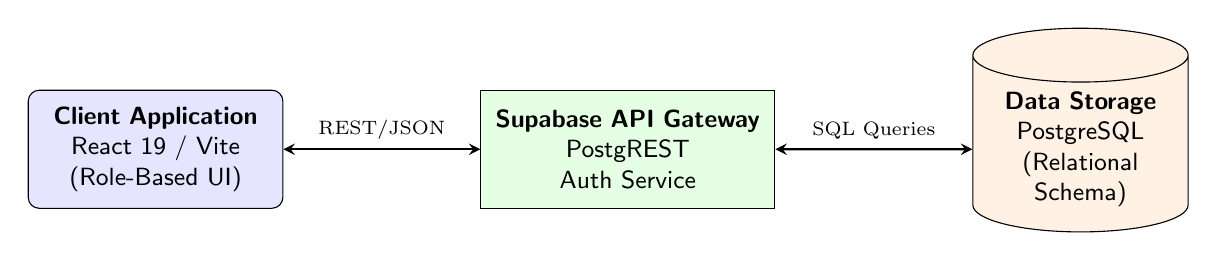
\begin{tikzpicture}[
    node distance=1.5cm and 2.5cm,
    client/.style={rectangle, draw, fill=blue!10, rounded corners, text width=3cm, align=center, minimum height=1.5cm, font=\sffamily\small},
    api/.style={rectangle, draw, fill=green!10, text width=3.5cm, align=center, minimum height=1.5cm, font=\sffamily\small},
    db/.style={cylinder, draw, shape border rotate=90, aspect=0.25, fill=orange!10, text width=2.5cm, align=center, minimum height=2cm, font=\sffamily\small},
    arrow/.style={draw, thick, <->, >=stealth}
]

% Nodes
\node[client] (react) {\textbf{Client Application}\\React 19 / Vite\\(Role-Based UI)};
\node[api, right=of react] (supabase) {\textbf{Supabase API Gateway}\\PostgREST\\Auth Service};
\node[db, right=of supabase] (postgres) {\textbf{Data Storage}\\PostgreSQL\\(Relational Schema)};

% Arrows
\draw[arrow] (react) -- (supabase) node[midway, above] {\scriptsize REST/JSON};
\draw[arrow] (supabase) -- (postgres) node[midway, above] {\scriptsize SQL Queries};

\end{tikzpicture}
\caption{High-Level System Architecture and Component Interaction}
\label{fig:system_architecture}
\end{figure}

The user interface is created with the ability to handle dense data interactions without a drop in performance. This is accomplished through the use of React's virtual DOM and TypeScript static type checking.

\subsection{Performance and Data Reliability}

For expensive operations like $O(N^2)$ clash detection, memoization of these logic-driven functions is done using the \texttt{useMemo} hook, such that these functions are run only if the data from the timetable has been modified. TypeScript is utilized for strict data interfaces, like \texttt{ParsedSlot}.

\begin{verbatim}
// Example TypeScript Interface for Solver Data Contracts
interface ParsedSlot {
    id: string;
    day: string;
    startTime: string;
    subjectCode: string;
    type: 'Lecture' | 'Tutorial' | 'Practical';
    roomName: string;
    section: string;
}
\end{verbatim}

%-----------------------------------
\section{Construction and Styling: Vite and Tailwind CSS}

Both the construction and styling processes are designed to facilitate fast iterations and immediate feedback loops.
\begin{itemize}
    \item \textbf{Vite:} Utilizes native ES Modules, enabling hot module replacement (HMR) almost instantaneously, which is essential during the optimization of grid generation algorithms.
    \item \textbf{Tailwind CSS:} The utility-based CSS framework makes it possible for the application to provide real-time styling feedback, such as a red border around conflicting sessions.
\end{itemize}

%-----------------------------------
\section{Back-end and Data Ingestion: Supabase}

Static files are replaced with a central PostgreSQL database provided by Supabase with referential integrity enforced using foreign keys.
\begin{itemize}
    \item \textbf{Heuristic Parsing:} The \texttt{xlsx} (SheetJS) package is utilized to parse institutional spreadsheets in their raw form. This information is interpreted using an in-house heuristic engine to derive its semantics, such as credit structures in the form of L-T-P and faculty mapping.
    \item \textbf{Authentication:} Authentication for administrators is achieved through Supabase Auth, which is implemented with state management through a global \texttt{AuthContext}.
\end{itemize}

%-----------------------------------
\section{Solver Engine: Architecture of Pure TypeScript}

The most important aspect of the current solution is its pure-TypeScript solver engine, which works directly in the browser. It doesn’t require any optimizations on the server side, enabling live generation of schedules. Solver consists of several modules:

\begin{itemize}
    \item \textbf{\texttt{dataPrep.ts}}: Breaks up high-level credits into individual sessions, applying the 2+1 rule of lectures.
    \item \textbf{\texttt{constraints.ts}}: Checks the solutions based on ten hard and three soft constraints.
    \item \textbf{\texttt{mutations.ts}}: Contains five different mutation operators, such as session day changing and Gaussian time shift.
    \item \textbf{\texttt{solver.ts}}: Works as a control center, managing the (1+1)-ES process, elitism, and restarts from stagnation.
    \item \textbf{\texttt{localSearch.ts}}: Applies local search operations to refine the schedule and resolve specific conflicts.
\end{itemize}

%-----------------------------------
\section{External Integration: Reporting and Exporting}

For workflow efficiency purposes, the system has the following integrations with external reporting systems:
\begin{itemize}
    \item \textbf{Google Sheets API:} Enables exportation of schedules to Google Drive in a frozen header format with session coloring.
    \item \textbf{PDF Output:} Makes use of \texttt{html-to-image} and \texttt{jsPDF} libraries for snapshot output of the timetable into PDF form.
\end{itemize}
% Chapter 4

\chapter{System Architecture and Design} % Main chapter title

\label{Chapter4} % For referencing the chapter elsewhere, use \ref{Chapter4}

%----------------------------------------------------------------------------------------

In this chapter, we walk through the structural design of the IIITA Timetabling System. We cover the overall application topology, the relational database schema, how we ingest data from Excel files, the solver module architecture, and the routing logic that ties everything together.

%-----------------------------------
\section{Application Topology}

Our system follows a classic three-tier architecture adapted for the modern web using a Backend-as-a-Service (BaaS) model.

\begin{itemize}
    \item \textbf{Client Tier (React SPA):} The frontend is a Single Page Application (SPA) responsible for all user interactions, data formatting, client-side clash detection, and PDF generation. It communicates asynchronously with the backend via secure REST API calls over HTTPS.
    \item \textbf{Backend Tier (Supabase):} Acting as the serverless backend, Supabase provides an auto-generated API gateway, handles user authentication, and interfaces directly with the underlying database.
    \item \textbf{Data Tier (PostgreSQL):} The relational database stores all normalized institutional data, including users, entities (rooms, subjects, professors), and the core timetable slots.
\end{itemize}

%-----------------------------------
\section{Database Schema Design}

A well-structured relational schema is paramount for a scheduling system to maintain data integrity and support complex queries. The database is heavily normalized to prevent data duplication and anomalies. The core schema comprises the following primary entities and relationships:

\subsection{Core Entities}

\begin{figure}[htbp]
\centering
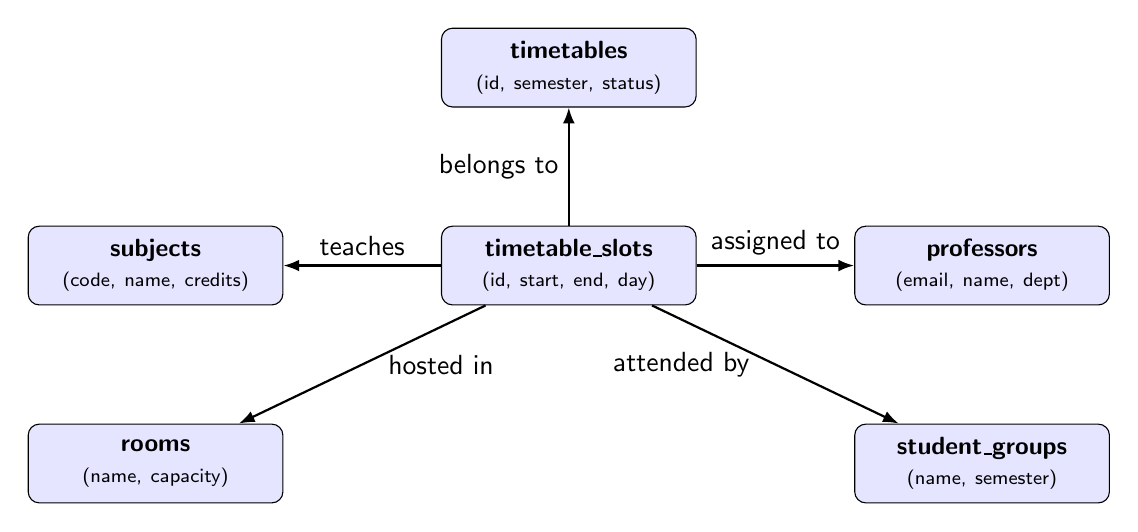
\begin{tikzpicture}[
    node distance=1.5cm and 2cm,
    entity/.style={rectangle, draw, fill=blue!10, rounded corners, text width=3cm, align=center, minimum height=1cm, font=\sffamily\small},
    relation/.style={diamond, draw, fill=orange!10, aspect=2, text width=2cm, align=center, font=\sffamily\scriptsize},
    line/.style={draw, thick, -{Latex[length=2mm]}},
    every node/.style={font=\sffamily}
]

% Nodes
\node[entity] (slots) {\textbf{timetable\_slots}\\ \scriptsize (id, start, end, day)};
\node[entity, above=of slots] (timetables) {\textbf{timetables}\\ \scriptsize (id, semester, status)};
\node[entity, left=of slots] (subjects) {\textbf{subjects}\\ \scriptsize (code, name, credits)};
\node[entity, right=of slots] (professors) {\textbf{professors}\\ \scriptsize (email, name, dept)};
\node[entity, below left=of slots] (rooms) {\textbf{rooms}\\ \scriptsize (name, capacity)};
\node[entity, below right=of slots] (groups) {\textbf{student\_groups}\\ \scriptsize (name, semester)};

% Relationships
\draw[line] (slots) -- (timetables) node[midway, left] {belongs to};
\draw[line] (slots) -- (subjects) node[midway, above] {teaches};
\draw[line] (slots) -- (professors) node[midway, above] {assigned to};
\draw[line] (slots) -- (rooms) node[midway, right, xshift=2mm] {hosted in};
\draw[line] (slots) -- (groups) node[midway, left, xshift=-2mm] {attended by};

\end{tikzpicture}
\caption{Simplified Entity-Relationship Diagram of the Core Schema}
\label{fig:er_diagram}
\end{figure}

\begin{itemize}
    \item \textbf{`timetables`:} Represents a specific iteration of a schedule (e.g., "B.Tech Sem 3 - Monsoon 2024"). It acts as the parent container for all scheduled slots. Attributes include the academic year, semester, publication status, and institutional break times (lunch start/end).
    \item \textbf{`subjects`:} Contains metadata for all offered courses. Attributes include the unique subject code, name, credit distribution (Lectures, Tutorials, Practicals), subject type (Core, Elective, Minor), and elective grouping data.
    \item \textbf{`professors`:} Stores faculty information, uniquely identified by email, alongside their departmental affiliation.
    \item \textbf{`rooms`:} Catalogs the physical infrastructure of the campus. Attributes include the unique room name (e.g., "CC-3-1001"), seating capacity, and room type (e.g., Lecture Hall, Computer Lab).
    \item \textbf{\texttt{student\_groups}:} Represents a specific cohort of students, defined by a unique combination of group name (e.g., "Sec A") and semester.
\end{itemize}

\subsection{The Central Hub: \texttt{timetable\_slots}}
The \texttt{timetable\_slots} table is the central junction of the schema. It represents a specific class occurrence in time and space. It acts as a massive join table, linking a specific \texttt{timetable\_id} to a \texttt{subject\_id}, \texttt{professor\_id}, \texttt{room\_id}, and \texttt{student\_group\_id}. 

Crucially, it also defines the temporal coordinates of the event, as detailed in Table~\ref{tab:schema_slots}.

\begin{table}[htbp]
\centering
\caption{Schema Specification for \texttt{timetable\_slots}}
\label{tab:schema_slots}
\renewcommand{\arraystretch}{1.4}
\begin{tabularx}{\textwidth}{@{} l l X @{}}
\toprule
\textbf{Column Name} & \textbf{Data Type} & \textbf{Description \& Constraints} \\
\midrule
\texttt{id} & \texttt{UUID} & Primary Key, auto-generated. \\
\texttt{timetable\_id} & \texttt{UUID} & Foreign Key referencing \texttt{timetables}. \\
\texttt{subject\_id} & \texttt{UUID} & Foreign Key referencing \texttt{subjects}. \\
\texttt{professor\_id} & \texttt{UUID} & Foreign Key referencing \texttt{professors}. \\
\texttt{room\_id} & \texttt{UUID} & Foreign Key referencing \texttt{rooms}. \\
\texttt{day\_of\_week} & \texttt{Integer} & $1 = \text{Monday}, \dots, 5 = \text{Friday}$. \\
\texttt{start\_time} & \texttt{VarChar} & 24-hour format (e.g., "09:00"). \\
\texttt{end\_time} & \texttt{VarChar} & 24-hour format (e.g., "11:00"). \\
\texttt{slot\_type} & \texttt{VarChar} & Enum: 'Lecture', 'Tutorial', 'Practical'. \\
\bottomrule
\end{tabularx}
\end{table}

\subsection{Generator and Solver Support Entities}
To support automated timetable generation, the schema includes mapping tables that define the constraints and requirements for specific semesters. These tables are actively used by the Generator Wizard and the solver engine:
\begin{itemize}
    \item \textbf{\texttt{semester\_clusters}:} Defines active academic clusters (e.g., Batch 2021, Semester 5, IT Department). The generator UI uses these clusters to scope the scheduling problem.
    \item \textbf{\texttt{cluster\_requirements}:} A many-to-many join table linking a \texttt{semester\_cluster} to the \texttt{subjects} that must be scheduled for that cohort. Includes \texttt{estimated\_enrollment} for room utilization optimization.
    \item \textbf{\texttt{professor\_expertise}:} A mapping table linking \texttt{professors} to \texttt{subjects} they are qualified to teach, along with a preference level. This is used by the auto-fill feature in the Generator Wizard to intelligently suggest professor assignments.
\end{itemize}

\subsection{Solver Data Model: Class Diagram}

Figure~\ref{fig:class_diagram} presents a UML class diagram of the solver's core data model, showing the relationships between the key TypeScript interfaces that drive the scheduling engine.

\begin{figure}[htbp]
\centering
\resizebox{\textwidth}{!}{%
\begin{tikzpicture}[
    class/.style={
        rectangle split, rectangle split parts=3,
        draw, thick, fill=blue!5,
        text width=5cm, align=center,
        font=\sffamily\scriptsize,
        rectangle split part fill={blue!15, white, white}
    },
    comp/.style={draw, thick, ->, >=Diamond[open], line width=0.8pt},
    assoc/.style={draw, thick, ->, >=stealth, dashed},
    note/.style={rectangle, draw, dashed, fill=yellow!10, text width=3cm, align=center, font=\sffamily\tiny, rounded corners}
]

% ClassSession
\node[class] (cs) {
    \textbf{ClassSession}
    \nodepart{second}
    \begin{tabular}{l}
    + id: number \\
    + subjectId: string \\
    + groupId: string \\
    + professorId: string \\
    + duration: number \\
    + slotType: enum \\
    + homeRoomIndex: number \\
    + isElective: boolean \\
    + basketName: string? \\
    + isLocked: boolean \\
    + lecturePairIndex: number \\
    \end{tabular}
    \nodepart{third}
    \textit{(immutable metadata)}
};

% Gene
\node[class, right=3cm of cs] (gene) {
    \textbf{Gene}
    \nodepart{second}
    \begin{tabular}{l}
    + day: 1--5 \\
    + startBucket: 1--8 \\
    + roomIndex: number \\
    \end{tabular}
    \nodepart{third}
    \textit{(scheduling decision)}
};

% SolverInput
\node[class, below=2.5cm of cs] (si) {
    \textbf{SolverInput}
    \nodepart{second}
    \begin{tabular}{l}
    + sessions: ClassSession[] \\
    + rooms: Room[] \\
    + numDays: 5 \\
    + numBuckets: 8 \\
    + config: SolverConfig \\
    \end{tabular}
    \nodepart{third}
    \textit{(solver entry point)}
};

% FitnessResult
\node[class, below=2.5cm of gene] (fr) {
    \textbf{FitnessResult}
    \nodepart{second}
    \begin{tabular}{l}
    + total: number \\
    + hardViolations: number \\
    + gapPenalty: number \\
    + roomUtilPenalty: number \\
    + profSameHalfPenalty: number \\
    + violationBreakdown: {...} \\
    \end{tabular}
    \nodepart{third}
    \textit{(evaluation output)}
};

% Solution type alias note
\node[note, above=0.8cm of gene] (sol) {
    \textbf{Solution} = Gene[] \\
    (1:1 with sessions)
};

% Relationships
\draw[comp] (si) -- node[left, font=\sffamily\tiny] {contains *} (cs);
\draw[comp] (sol) -- node[right, font=\sffamily\tiny] {contains *} (gene);
\draw[assoc] (cs) -- node[above, font=\sffamily\tiny] {maps 1:1} (gene);
\draw[assoc] (si.east) -- node[below, font=\sffamily\tiny] {evaluate() $\to$} (fr.west);

\end{tikzpicture}
}%
\caption{UML Class Diagram of the Solver Data Model}
\label{fig:class_diagram}
\end{figure}

%-----------------------------------
\section{The Data Ingestion Pipeline}

A major architectural feature of the system is its ability to ingest unstructured data. The transition from an administrator's raw Excel file to normalized database records follows a strict pipeline managed by the \texttt{TimetableImporter} module:

\begin{figure}[htbp]
\centering
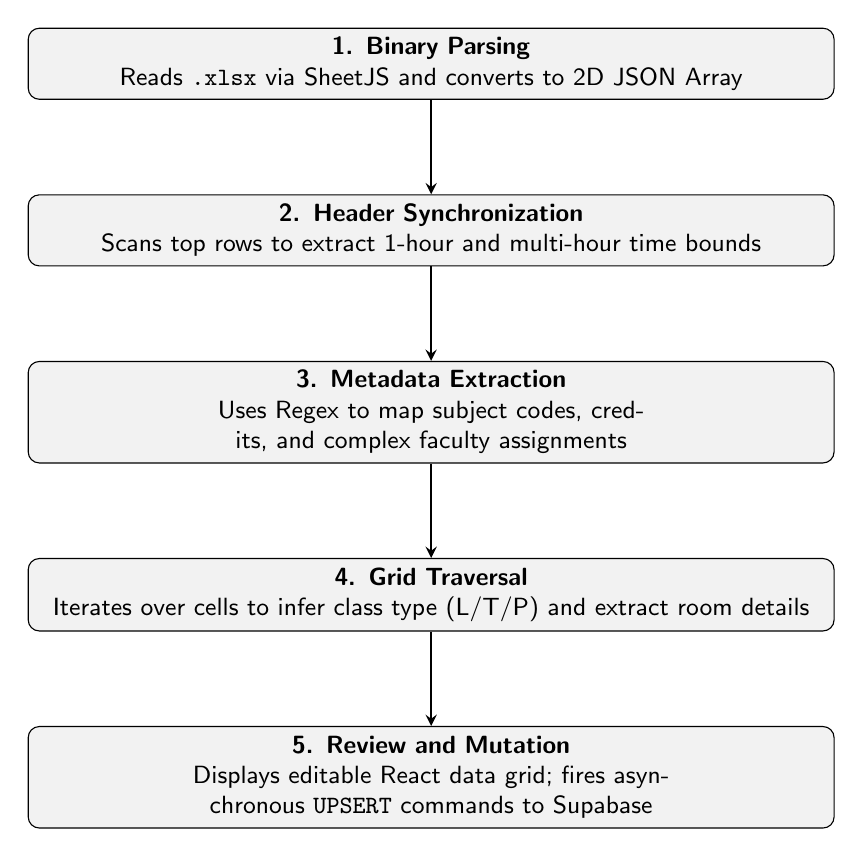
\begin{tikzpicture}[
    node distance=1.2cm,
    block/.style={rectangle, draw, fill=gray!10, text width=10cm, align=center, rounded corners, minimum height=0.8cm, font=\sffamily\small},
    arrow/.style={draw, thick, ->, >=stealth}
]

\node[block] (step1) {\textbf{1. Binary Parsing}\\Reads \texttt{.xlsx} via SheetJS and converts to 2D JSON Array};
\node[block, below=of step1] (step2) {\textbf{2. Header Synchronization}\\Scans top rows to extract 1-hour and multi-hour time bounds};
\node[block, below=of step2] (step3) {\textbf{3. Metadata Extraction}\\Uses Regex to map subject codes, credits, and complex faculty assignments};
\node[block, below=of step3] (step4) {\textbf{4. Grid Traversal}\\Iterates over cells to infer class type (L/T/P) and extract room details};
\node[block, below=of step4] (step5) {\textbf{5. Review and Mutation}\\Displays editable React data grid; fires asynchronous \texttt{UPSERT} commands to Supabase};

\draw[arrow] (step1) -- (step2);
\draw[arrow] (step2) -- (step3);
\draw[arrow] (step3) -- (step4);
\draw[arrow] (step4) -- (step5);

\end{tikzpicture}
\caption{Data Ingestion Pipeline for Excel Timetables}
\label{fig:parsing_pipeline}
\end{figure}

\begin{enumerate}
    \item \textbf{Binary Parsing:} The user uploads an `.xlsx` file. The `xlsx` library reads the binary stream and converts the active spreadsheet into a two-dimensional JSON array.
    \item \textbf{Header Synchronization:} The heuristic engine scans the top rows to identify the time boundary headers. It extracts standard 1-hour blocks (e.g., 9:00-10:00) and multi-hour blocks.
    \item \textbf{Metadata Extraction:} The engine locates the "Course Code / Faculties" section of the spreadsheet. It applies Regular Expressions (Regex) to map subject codes to full names and extracts the L-T-P-S credit structures. It also parses complex faculty assignment strings (e.g., identifying that "Prof. X" teaches "Sec A \& B" while "Prof. Y" teaches "Sec C").
    \item \textbf{Grid Traversal and Extraction:} The engine iterates over the main timetable grid. For each cell, it:
    \begin{itemize}
        \item Identifies the current day from the leftmost column.
        \item Identifies the time bounds from the column header.
        \item Extracts the subject code, infers the class type (L/T/P) based on cell coloring or text markers, and extracts room and section assignments.
    \end{itemize}
    \item \textbf{Review and Mutation:} The extracted raw data is presented to the administrator in an editable React data grid. Upon confirmation, the application fires a sequence of asynchronous \texttt{UPSERT} commands to Supabase, ensuring that all necessary entities (professors, rooms, subjects) exist before performing a bulk \texttt{INSERT} into the \texttt{timetable\_slots} table.
\end{enumerate}

%-----------------------------------
\section{View Routing and State Management}

The application does not utilize a traditional URL-based router (like React Router). Instead, it employs state-based view switching managed by the root `App.tsx` component. 

A central state variable, `currentView`, dictates which heavy component is mounted into the main viewing area. The available views are:
\begin{itemize}
    \item \texttt{import}: Mounts the \texttt{TimetableImporter}.
    \item \texttt{generator}: Mounts the multi-step \texttt{GeneratorView} wizard for automated timetable creation.
    \item \texttt{editor}: Mounts the interactive \texttt{EditorView} for drag-and-drop timetable refinement with LNS auto-fix.
    \item \texttt{student}: Mounts the \texttt{TimetableViewer} (All Students administrative view).
    \item \texttt{prof}: Mounts the \texttt{ProfessorTimetableViewer}.
    \item \texttt{room}: Mounts the \texttt{RoomTimetableViewer}.
    \item \texttt{master-room}: Mounts the campus-wide \texttt{MasterRoomViewer}.
    \item \texttt{free-room}: Mounts the \texttt{FreeRoomViewer}.
    \item \texttt{report-card}: Mounts the \texttt{ReportCardView}.
\end{itemize}

This architecture ensures that only the data required for the active view is fetched from the database, minimizing unnecessary network traffic. Custom React hooks, notably \texttt{useGeneratorData} and \texttt{useEditorData}, manage the fetching and caching of complex relational data required by these components, abstracting the Supabase query syntax away from the presentation layer.
 
% Chapter 5

\chapter{Implementation and Results} % Main chapter title

\label{Chapter5}

%----------------------------------------------------------------------------------------

\section{Introduction to the Optimization Engine}

The transition from data ingestion to the core solver introduces a highly constrained NP-hard optimization problem. The IIITA Timetabling System models this challenge mathematically, solving it via client-side heuristics. Rather than relying on traditional deterministic approaches which fail to scale, the system employs an evolutionary search mechanism. The engine processes high-dimensional inputs---comprising student cohorts, faculty assignments, and spatial capacities---and systematically navigates a vast, discontinuous search space to identify a globally optimal, conflict-free schedule.

\begin{figure}[htbp]
\centering
\resizebox{\textwidth}{!}{%
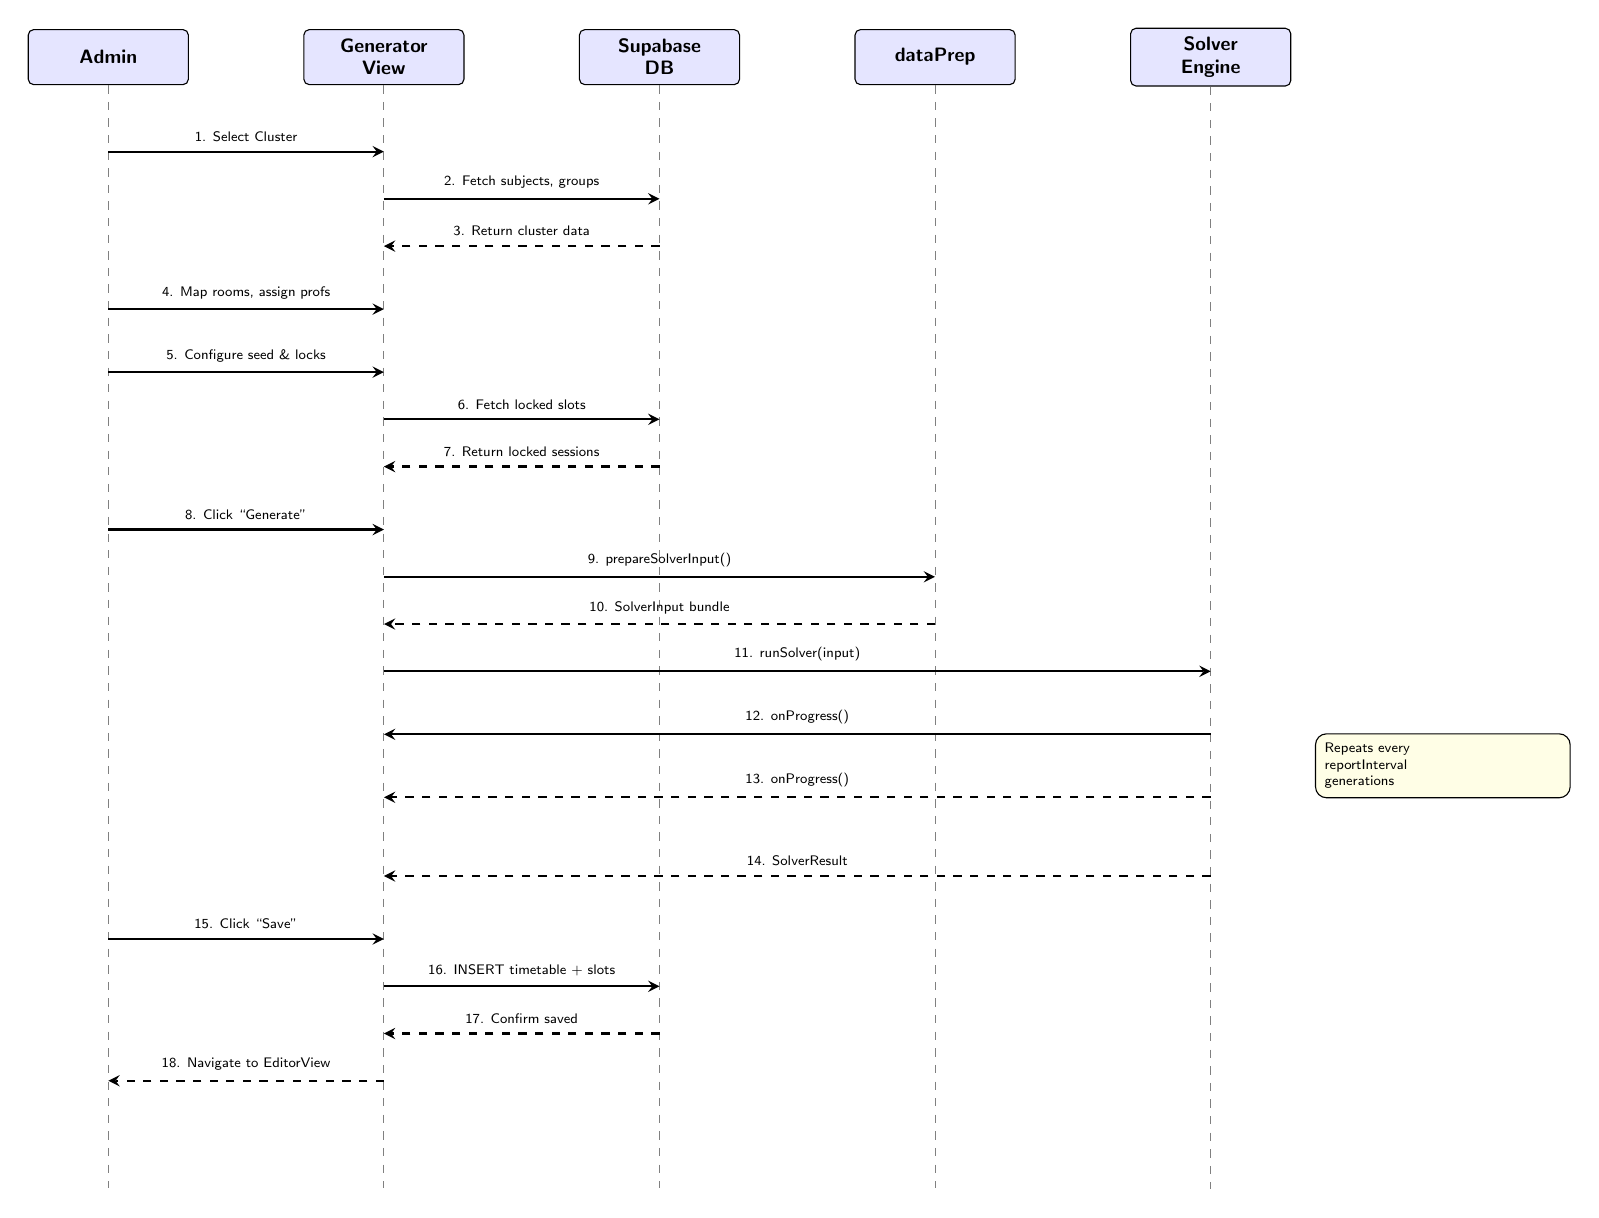
\begin{tikzpicture}[
    actor/.style={rectangle, draw, fill=blue!10, text width=1.8cm, align=center, font=\sffamily\scriptsize, minimum height=0.7cm, rounded corners=2pt},
    lifeline/.style={dashed, gray},
    msg/.style={->, >=stealth, thick, font=\sffamily\tiny},
    rmsg/.style={->, >=stealth, thick, dashed, font=\sffamily\tiny},
    activation/.style={fill=blue!8, draw, minimum width=0.3cm},
    note/.style={rectangle, draw, fill=yellow!10, text width=3cm, align=left, font=\sffamily\tiny, rounded corners}
]

% Actors
\node[actor] (admin) at (0,0) {\textbf{Admin}};
\node[actor] (gen) at (3.5,0) {\textbf{Generator\\View}};
\node[actor] (db) at (7,0) {\textbf{Supabase\\DB}};
\node[actor] (prep) at (10.5,0) {\textbf{dataPrep}};
\node[actor] (solver) at (14,0) {\textbf{Solver\\Engine}};

% Lifelines
\foreach \x in {admin, gen, db, prep, solver} {
    \draw[lifeline] (\x.south) -- ++(0,-14);
}

% Messages
\draw[msg] (0,-1.2) -- node[above] {1. Select Cluster} (3.5,-1.2);
\draw[msg] (3.5,-1.8) -- node[above] {2. Fetch subjects, groups} (7,-1.8);
\draw[rmsg] (7,-2.4) -- node[above] {3. Return cluster data} (3.5,-2.4);

\draw[msg] (0,-3.2) -- node[above] {4. Map rooms, assign profs} (3.5,-3.2);

\draw[msg] (0,-4.0) -- node[above] {5. Configure seed \& locks} (3.5,-4.0);
\draw[msg] (3.5,-4.6) -- node[above] {6. Fetch locked slots} (7,-4.6);
\draw[rmsg] (7,-5.2) -- node[above] {7. Return locked sessions} (3.5,-5.2);

\draw[msg] (0,-6.0) -- node[above] {8. Click ``Generate''} (3.5,-6.0);
\draw[msg] (3.5,-6.6) -- node[above] {9. prepareSolverInput()} (10.5,-6.6);
\draw[rmsg] (10.5,-7.2) -- node[above] {10. SolverInput bundle} (3.5,-7.2);

\draw[msg] (3.5,-7.8) -- node[above] {11. runSolver(input)} (14,-7.8);

% Solver loop
\draw[msg] (14,-8.6) -- node[above] {12. onProgress()} (3.5,-8.6);
\node[note, right=0.3cm of solver, yshift=-9cm] (loop) {Repeats every\\reportInterval\\generations};
\draw[rmsg] (14,-9.4) -- node[above] {13. onProgress()} (3.5,-9.4);

\draw[rmsg] (14,-10.4) -- node[above] {14. SolverResult} (3.5,-10.4);

\draw[msg] (0,-11.2) -- node[above] {15. Click ``Save''} (3.5,-11.2);
\draw[msg] (3.5,-11.8) -- node[above] {16. INSERT timetable + slots} (7,-11.8);
\draw[rmsg] (7,-12.4) -- node[above] {17. Confirm saved} (3.5,-12.4);
\draw[rmsg] (3.5,-13.0) -- node[above] {18. Navigate to EditorView} (0,-13.0);

\end{tikzpicture}
}%
\caption{Sequence Diagram: End-to-End Intelligent Generator Workflow}
\label{fig:generator_sequence}
\end{figure}

\section{Mathematical Representation of the Schedule}

To facilitate computational optimization, the schedule is encoded into a specific data structure known as a \textit{Chromosome}. The solver models a complete timetable $S$ as an ordered array of \textit{genes}. Each gene $g_i \in S$ encodes the precise scheduling decision for the $i$-th class session, mapping it to a spatial and temporal coordinate. 

Formally, a gene is defined as a tuple:
\begin{equation}
    g_i = (d_i, t_i, r_i)
\end{equation}
where:
\begin{itemize}
    \item $d_i \in \{1, 2, 3, 4, 5\}$ represents the day of the week (Monday through Friday).
    \item $t_i \in \{1, 2, \dots, 8\}$ represents the discrete start time slot (each slot corresponding to one hour, from 08:50 to 18:30).
    \item $r_i \in \mathcal{R}$ is the index into the array of available physical rooms.
\end{itemize}

Each gene is invariably linked to an immutable \texttt{ClassSession} object that contains the session's metadata: the specific subject identifier, the student group $G_i$, the assigned professor $p_i$, the duration $D_i$, and the specific slot type (Lecture, Tutorial, or Practical).

\section{Mathematical Formulation of Constraints}

The optimization objective is governed by a composite fitness function that evaluates both the feasibility and the quality of the candidate solution $S$.

\subsection{Hard Constraints (The Feasibility Space)}

Hard constraints define the boundary of feasible solutions. A schedule is strictly invalid if any hard constraint is violated. For two distinct sessions $i$ and $j$, we define the temporal overlap condition as:
\begin{equation}
    \text{overlap}(t_i, t_j) = \begin{cases} 
      1 & \text{if } \max(t_i, t_j) \le \min(t_i + D_i - 1, t_j + D_j - 1) \\
      0 & \text{otherwise}
   \end{cases}
\end{equation}

The engine enforces the following critical hard penalties:
\begin{itemize}
    \item \textbf{Professor Overlap Penalty:} A professor $p$ cannot be physically present in two different locations at time $t$. 
    \begin{equation}
        \sum_{i \neq j} \mathbb{I}(p_i = p_j \land d_i = d_j \land \text{overlap}(t_i, t_j)) = 0
    \end{equation}

    \item \textbf{Student Group Overlap Penalty:} A specific student cohort $G$ cannot attend two distinct subjects simultaneously. (Concurrent sessions from the same synchronized elective basket are mathematically exempted).
    \begin{equation}
        \sum_{i \neq j} \mathbb{I}(G_i = G_j \land d_i = d_j \land \text{overlap}(t_i, t_j) \land \neg \text{SameBasket}(i, j)) = 0
    \end{equation}

    \item \textbf{Room Clash Penalty:} A physical room $r$ can host at most one session at any given time.
    \begin{equation}
        \sum_{i \neq j} \mathbb{I}(r_i = r_j \land d_i = d_j \land \text{overlap}(t_i, t_j)) = 0
    \end{equation}

    \item \textbf{Lunch Boundary Enforcement:} Sessions cannot cross the designated lunch break ($B_{lunch}$ from 13:00 to 14:30, bounded between slot 4 and 5). 
    \begin{equation}
        \forall i \in S, \quad [t_i, t_i + D_i - 1] \cap B_{lunch} = \emptyset
    \end{equation}

    \item \textbf{L-T-P ``Chunking'' (The 2+1 Rule):} For core courses with $L \ge 2$ credits, the algorithm mathematically forces the contact hours into a contiguous 2-hour block and subsequent 1-hour blocks, distributed across distinct days. Let $\mathcal{L}_c$ be the set of lecture sessions for subject $c$:
    \begin{equation}
        \exists! k \in \mathcal{L}_c : D_k = 2 \quad \text{and} \quad \forall j \in \mathcal{L}_c \setminus \{k\}, D_j = 1
    \end{equation}
    \begin{equation}
        \forall i, j \in \mathcal{L}_c, \ i \neq j \implies d_i \neq d_j
    \end{equation}
\end{itemize}

\begin{table}[htbp]
\centering
\caption{Hard Constraints Enforced by the Solver}
\label{tab:hard_constraints}
\renewcommand{\arraystretch}{1.4}
\begin{tabularx}{\textwidth}{@{} c l X @{}}
\toprule
\textbf{\#} & \textbf{Constraint Name} & \textbf{Description} \\
\midrule
1 & Time Boundary & A session must not extend beyond slot 8 (18:30). \\
2 & Break/Lunch Crossing & A multi-slot session must not span across a break boundary (slots 2$\to$3 or 4$\to$5). \\
3 & Room Non-Overlap & At most one session may occupy a given room at any (day, slot). \\
4 & Professor Non-Overlap & A professor can teach at most one session at any given slot. No elective exemption. \\
5 & Group Non-Overlap & A student group can attend at most one session per slot. Elective--elective pairs and same-basket pairs are exempt. \\
6 & Elective Basket Sync & Synced baskets (HSMC, MDM) must share the same (day, slot). No two different baskets may share a slot (global anti-clash). \\
7 & Lab Room & Practical sessions must be assigned to rooms with type ``Lab''. \\
8 & WMC-Section Overlap & A whole-batch (WMC) session cannot occupy the same slot as any section-level session. \\
9 & Home Room & Core lectures and tutorials must be placed in their assigned home room. \\
10 & 2+1 Lecture Format & The double-lecture block and single-lectures for the same subject+group must be on different days. \\
\bottomrule
\end{tabularx}
\end{table}

\subsection{Soft Constraints (The Quality Space)}

Once the solution space is feasible, the engine optimizes for schedule quality by minimizing soft penalties.

\begin{itemize}
    \item \textbf{Minimizing Student Gaps:} The engine minimizes idle slots between a cohort's first and last class on any given day. Let $\mathcal{T}_{g,d}$ be the set of all active time slots for student group $g$ on day $d$. The gap penalty $G(S)$ is:
    \begin{equation}
        G(S) = \sum_{g} \sum_{d} \left( (\max(\mathcal{T}_{g,d}) - \min(\mathcal{T}_{g,d}) + 1) - |\mathcal{T}_{g,d}| \right)
    \end{equation}

    \item \textbf{Room Capacity Optimization:} The system matches class enrollment $c_i$ to room capacity $K_{r_i}$. Let the utilization ratio be $u_i = c_i / K_{r_i}$. Given optimal thresholds $\alpha = 0.6$ and $\beta = 1.2$, the room utilization penalty $R(S)$ is formulated as:
    \begin{equation}
        R(S) = \sum_{i} \left( \max(0, \alpha - u_i) + \max(0, u_i - \beta) \right)
    \end{equation}
\end{itemize}

\section{The (1+1) Evolution Strategy Solver}

The optimization engine is powered by a (1+1) Evolution Strategy (ES) algorithm. It relies on iterative stochastic perturbations and adaptive mutation rates to navigate the constrained schedule space.

\subsection{Strict Elitism}

The algorithm employs a strictly elitist selection mechanism. In each generation, a parent solution $S_{parent}$ undergoes mutation to produce a single offspring $S_{child}$. The offspring replaces the parent if and only if its total fitness score is less than or equal to the parent's score:
\begin{equation}
    S_{parent}^{(t+1)} = \begin{cases} 
      S_{child} & \text{if } f(S_{child}) \le f(S_{parent}^{(t)}) \\
      S_{parent}^{(t)} & \text{otherwise}
   \end{cases}
\end{equation}
This greediness guarantees that the solver never loses ground on hard constraint feasibility.

\subsection{Mutation Operators}

To generate $S_{child}$, the engine selects a subset of mutable sessions and applies highly stochastic operators:
\begin{itemize}
    \item \textbf{Gaussian Time Shifts:} The start time $t_i$ is perturbed using Gaussian noise scaled by variance $\sigma$:
    \begin{equation}
        t_i^{(new)} = t_i + \lfloor \mathcal{N}(0, \sigma^2) \rceil
    \end{equation}
    \item \textbf{Type-Aware Room Reassignments:} A session is moved to a randomly selected room $r_k \in \mathcal{R}$ that strictly matches its required architectural type (e.g., Lab vs. Lecture Hall).
    \item \textbf{Targeted Swaps:} Two sessions $i$ and $j$ of identical duration exchange their spatial-temporal coordinates, effectively jumping out of local minima without increasing the overall density.
\end{itemize}

\subsection{Adaptive Variance (The Brain)}

To dynamically balance global exploration and local exploitation, the solver implements Rechenberg's 1/5th Success Rule. The mutation strength $\sigma$ is adapted every $W = 50$ generations based on the success rate $p_s$ (the ratio of offspring that successfully improved or matched fitness).
\begin{equation}
    \sigma \leftarrow
    \begin{cases}
        \sigma \times 1.22 & \text{if } p_s > 0.20 \quad \text{(Search wider)} \\
        \sigma \times 0.82 & \text{if } p_s < 0.20 \quad \text{(Search finer)} \\
        \sigma & \text{otherwise}
    \end{cases}
\end{equation}

\subsection{Stagnation Recovery}

In highly dense optimization landscapes, the algorithm may converge to a deep local optimum (a plateau). The engine mathematically tracks this stagnation. If $S_{parent}$ fails to improve for 15,000 consecutive generations, a stagnation recovery protocol is triggered. The current candidate is discarded, and maximum entropy is injected by generating a completely new randomized initial timetable.

\begin{figure}[htbp]
\centering
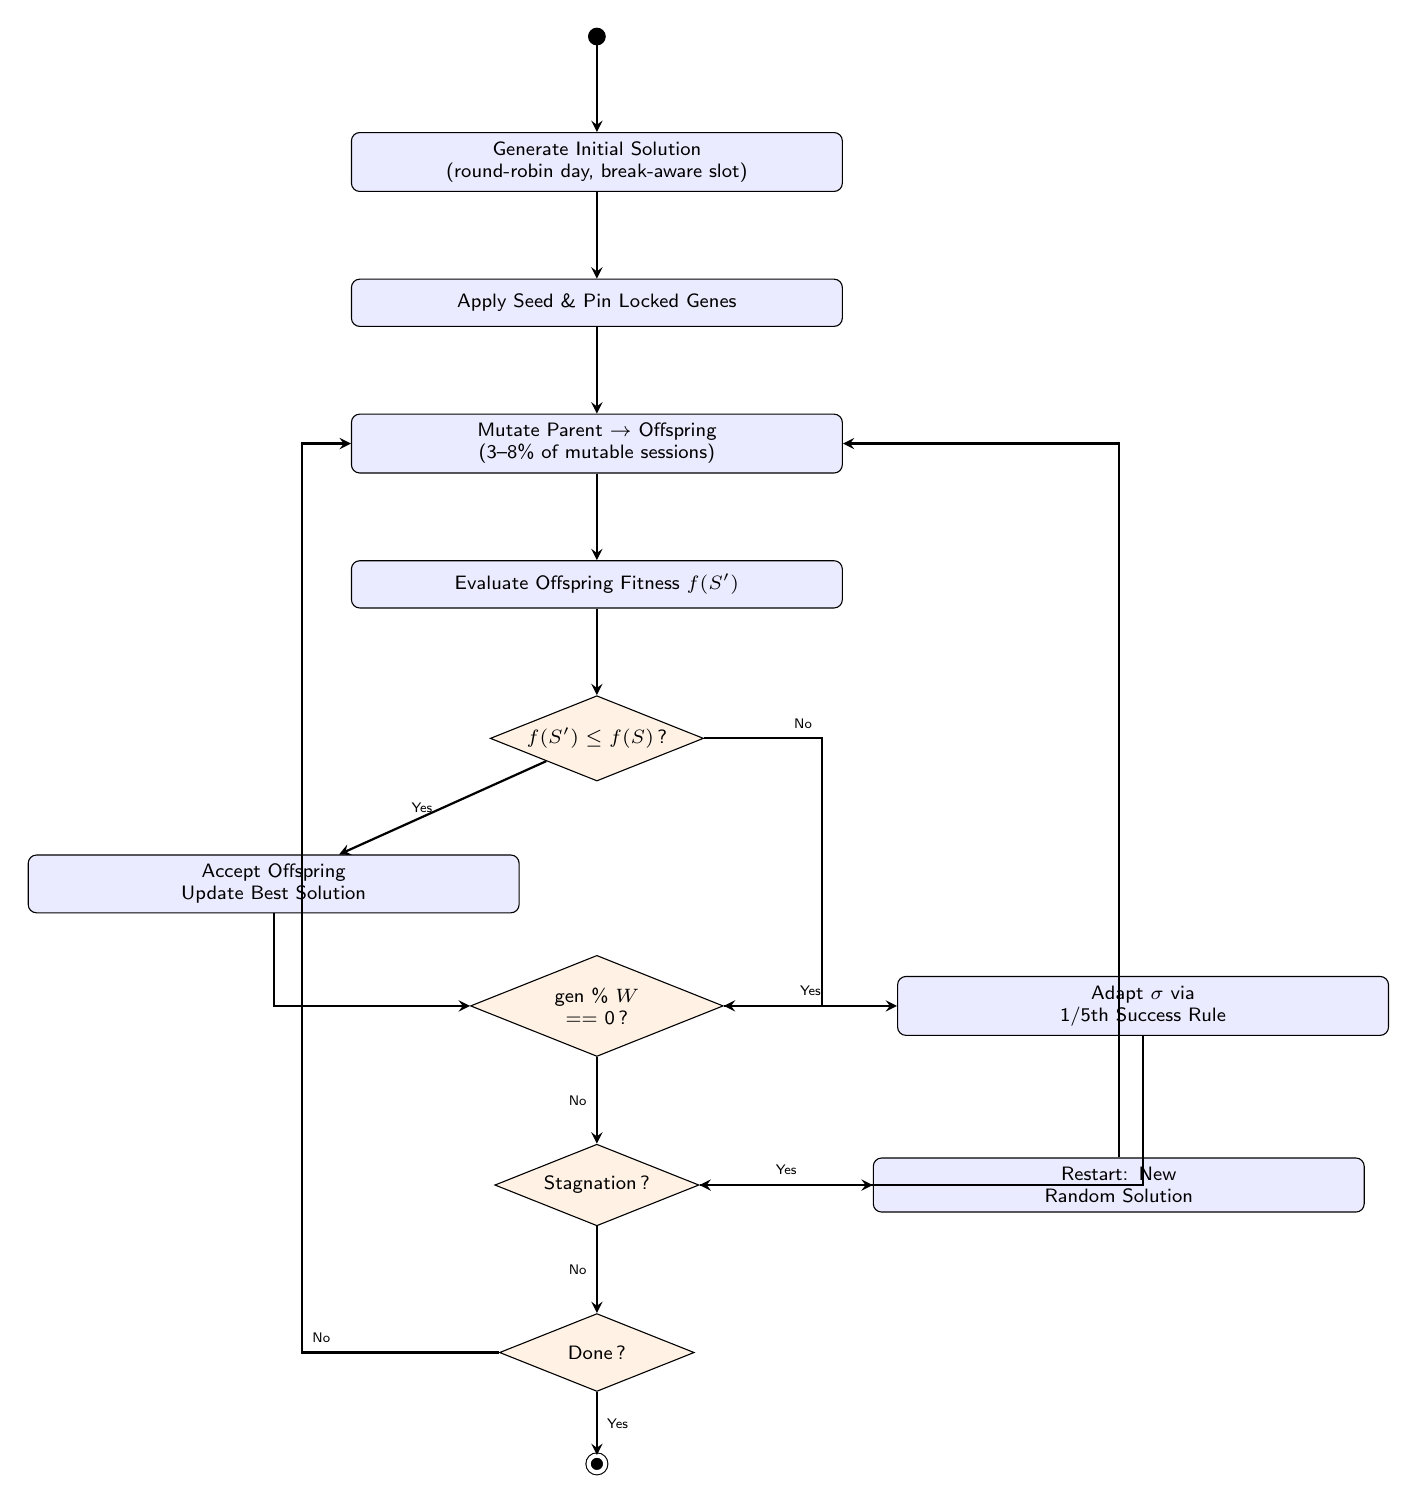
\begin{tikzpicture}[
    node distance=1.1cm,
    start/.style={draw, circle, fill=black, minimum size=6pt, inner sep=0pt},
    stop/.style={draw, circle, fill=black, minimum size=6pt, inner sep=0pt, double, double distance=1.5pt},
    action/.style={draw, rectangle, fill=blue!8, rounded corners=3pt, text width=6cm, align=center, font=\sffamily\scriptsize, minimum height=0.6cm},
    decision/.style={draw, diamond, aspect=2.5, fill=orange!10, text width=1.8cm, align=center, font=\sffamily\scriptsize, inner sep=1pt},
    arrow/.style={draw, thick, ->, >=stealth, font=\sffamily\tiny}
]

\node[start] (s) {};
\node[action, below=of s] (init) {Generate Initial Solution\\(round-robin day, break-aware slot)};
\node[action, below=of init] (seed) {Apply Seed \& Pin Locked Genes};
\node[action, below=of seed] (mutate) {Mutate Parent $\to$ Offspring\\(3--8\% of mutable sessions)};
\node[action, below=of mutate] (eval) {Evaluate Offspring Fitness $f(S')$};
\node[decision, below=of eval] (accept) {$f(S') \leq f(S)$\,?};
\node[action, below left=1.2cm and 0.3cm of accept] (yes) {Accept Offspring\\Update Best Solution};
\node[decision, below=2.2cm of accept] (sigma) {gen \% $W$ == 0\,?};
\node[action, right=2.2cm of sigma] (adapt) {Adapt $\sigma$ via\\1/5th Success Rule};
\node[decision, below=of sigma] (stag) {Stagnation\,?};
\node[action, right=2.2cm of stag] (restart) {Restart: New\\Random Solution};
\node[decision, below=of stag] (term) {Done\,?};
\node[stop, below=0.8cm of term] (e) {};

\draw[arrow] (s) -- (init);
\draw[arrow] (init) -- (seed);
\draw[arrow] (seed) -- (mutate);
\draw[arrow] (mutate) -- (eval);
\draw[arrow] (eval) -- (accept);
\draw[arrow] (accept) -- node[left] {Yes} (yes);
\draw[arrow] (accept.east) -- ++(1.5,0) node[above left, font=\sffamily\tiny] {No} |- (sigma);
\draw[arrow] (yes) |- (sigma);
\draw[arrow] (sigma) -- node[above] {Yes} (adapt);
\draw[arrow] (sigma) -- node[left] {No} (stag);
\draw[arrow] (adapt) |- (stag);
\draw[arrow] (stag) -- node[above] {Yes} (restart);
\draw[arrow] (stag) -- node[left] {No} (term);
\draw[arrow] (restart) |- (mutate);
\draw[arrow] (term.west) -- ++(-2.5,0) node[above right, font=\sffamily\tiny] {No} |- (mutate);
\draw[arrow] (term) -- node[right] {Yes} (e);

\end{tikzpicture}
\caption{Activity Diagram: (1+1)-ES Solver Execution Flow}
\label{fig:solver_activity}
\end{figure}

\section{Interactive Editor \& Large Neighbourhood Search (LNS)}

The user interface functions primarily as an engineering tool designed for granular control over the algorithmic output. When manual drag-and-drop actions introduce systemic conflicts, an integrated Large Neighbourhood Search (LNS) is deployed to repair the grid.

The ``Auto-Fix'' feature applies a destroy-and-repair heuristic. Instead of recalculating the entire grid, it isolates the localized clashing subset $C \subseteq S$. The LNS algorithm iterates up to 1,500 times, randomly selecting a session $i \in C$, applying stochastic mutations (relocation, time shifts, or swaps), and evaluating the local differential fitness. If a localized mutation resolves the clash without violating surrounding sessions, the repair is committed.

\begin{figure}[htbp]
\centering
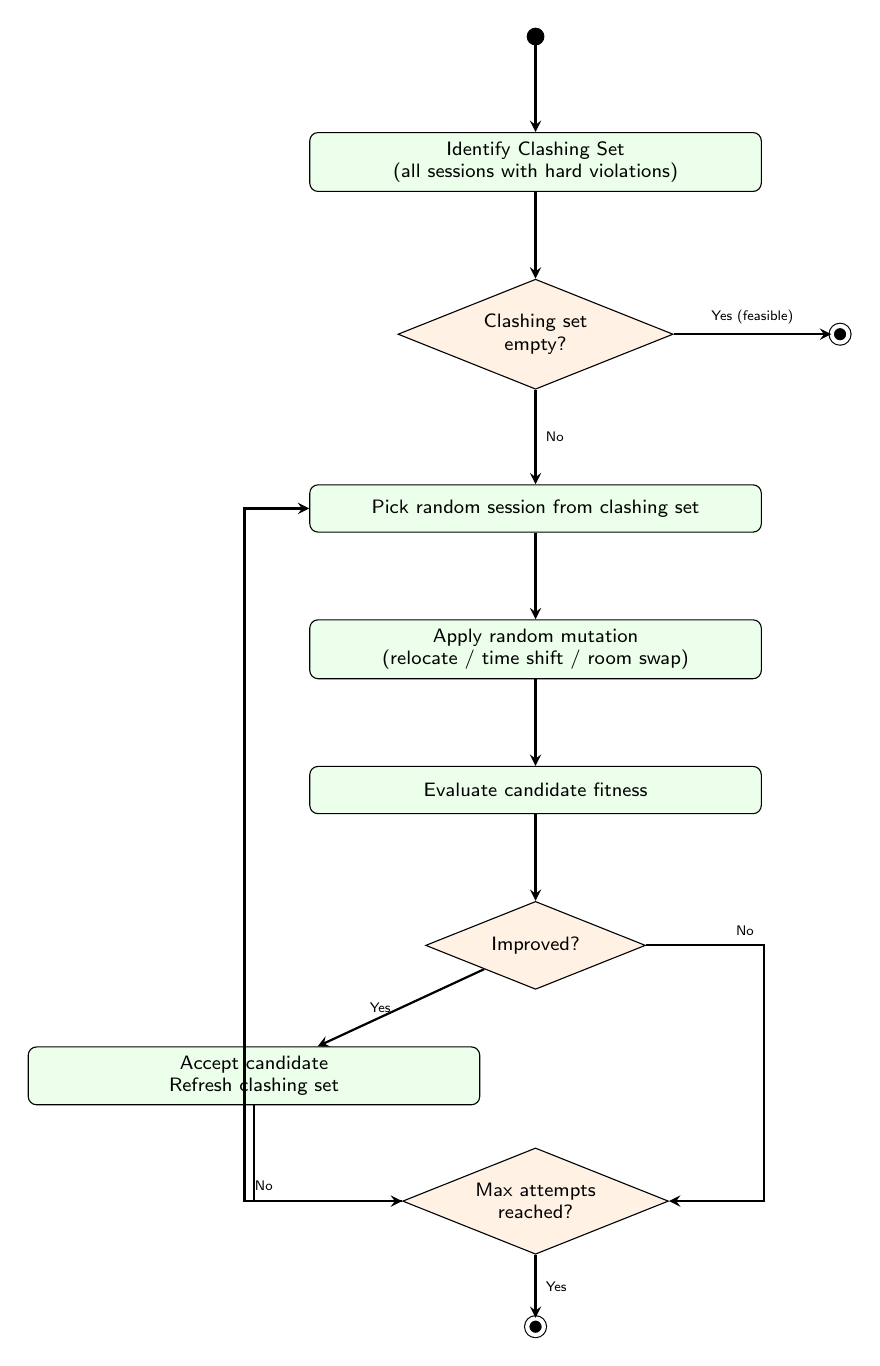
\begin{tikzpicture}[
    node distance=1.1cm,
    start/.style={draw, circle, fill=black, minimum size=6pt, inner sep=0pt},
    stop/.style={draw, circle, fill=black, minimum size=6pt, inner sep=0pt, double, double distance=1.5pt},
    action/.style={draw, rectangle, fill=green!8, rounded corners=3pt, text width=5.5cm, align=center, font=\sffamily\scriptsize, minimum height=0.6cm},
    decision/.style={draw, diamond, aspect=2.5, fill=orange!10, text width=2cm, align=center, font=\sffamily\scriptsize, inner sep=1pt},
    arrow/.style={draw, thick, ->, >=stealth, font=\sffamily\tiny}
]

\node[start] (s) {};
\node[action, below=of s] (find) {Identify Clashing Set\\(all sessions with hard violations)};
\node[decision, below=of find] (empty) {Clashing set\\empty?};
\node[action, below=1.2cm of empty] (pick) {Pick random session from clashing set};
\node[action, below=of pick] (mut) {Apply random mutation\\(relocate / time shift / room swap)};
\node[action, below=of mut] (ev) {Evaluate candidate fitness};
\node[decision, below=of ev] (better) {Improved?};
\node[action, below left=1cm and 0cm of better] (acc) {Accept candidate\\Refresh clashing set};
\node[decision, below=2cm of better] (maxiter) {Max attempts\\reached?};
\node[stop, right=2cm of empty] (done1) {};
\node[stop, below=0.8cm of maxiter] (done2) {};

\draw[arrow] (s) -- (find);
\draw[arrow] (find) -- (empty);
\draw[arrow] (empty) -- node[right] {No} (pick);
\draw[arrow] (empty) -- node[above] {Yes (feasible)} (done1);
\draw[arrow] (pick) -- (mut);
\draw[arrow] (mut) -- (ev);
\draw[arrow] (ev) -- (better);
\draw[arrow] (better) -- node[left] {Yes} (acc);
\draw[arrow] (better.east) -- ++(1.5,0) node[above left, font=\sffamily\tiny] {No} |- (maxiter);
\draw[arrow] (acc) |- (maxiter);
\draw[arrow] (maxiter) -- node[right] {Yes} (done2);
\draw[arrow] (maxiter.west) -- ++(-2,0) node[above right, font=\sffamily\tiny] {No} |- (pick);

\end{tikzpicture}
\caption{Activity Diagram: LNS Destroy-and-Repair Auto-Fix}
\label{fig:lns_activity}
\end{figure}

\section{Results and Application Features}

The implementation of the optimization engine drastically reduces the administrative overhead. By executing entirely client-side, the system achieves feasibility rapidly, circumventing backend server latencies.

\subsection{Algorithmic Convergence}

The solver demonstrates rapid convergence. The heavily weighted hard penalties force the evolution strategy to prioritize feasibility before aggressively optimizing the soft quality metrics.

`[Insert Image: Fitness Score vs. Generations Graph]`

\subsection{The Interactive Drag-and-Drop Grid}

The primary workspace visualizes the temporal matrix. It calculates multi-dimensional clashes in real-time, surfacing spatial and temporal overlaps through distinct programmatic warnings.

`[Insert Image: Main UI Grid showing Clashes]`

\subsection{LNS Auto-Fix Execution}

When administrators execute the LNS repair routine, the interface explicitly highlights the target neighbourhood and dynamically resolves overlapping nodes without destabilizing the optimized framework.

`[Insert Image: UI highlighting Auto-Fix suggestions]`

\subsection{Export and PDF Generation}

The final scheduling matrix is programmatically serialized into a high-fidelity PDF, leveraging DOM capture logic to bypass CSS layout constraints, ensuring the complete multidimensional array is rendered cleanly.

`[Insert Image: Final PDF Timetable Output]`

%-----------------------------------
\section{Dynamic Time Grid Generation}

A significant challenge in displaying timetables is the variability of time slots. Hardcoding a static grid (e.g., exactly ten 1-hour slots from 9:00 AM to 7:00 PM) results in wasted visual space when classes end early, and fails to accommodate non-standard time ranges (such as a 1.5-hour class).

To solve this, all viewer components in the system implement a \textbf{Dynamic Time Column Generator algorithm}.
When a timetable is selected, the system fetches all associated \texttt{timetable\_slots}. The algorithm then executes the following steps:
\begin{enumerate}
    \item Extracts all unique \texttt{start\_time} and \texttt{end\_time} strings from the raw slot data.
    \item Injects hardcoded institutional break times: \texttt{10:50} to \texttt{11:00} (Morning Break) and \texttt{13:00} to \texttt{14:30} (Lunch Break).
    \item Sorts all extracted timestamps chronologically to create an array of discrete time boundaries.
    \item Iterates through adjacent pairs of boundaries to generate standard columns.
    \item Filters out any generated columns that fall entirely within the lunch or break periods, or that contain absolutely zero scheduled classes.
\end{enumerate}

The result is a highly responsive grid that only displays columns for active periods, maximizing screen real estate and improving readability.

%-----------------------------------
\section{Multi-Dimensional Clash Detection Algorithm}

One of the most critical administrative features is the automated detection of scheduling conflicts. The `TimetableViewer` component implements a robust $O(N^2)$ algorithm that compares every slot against every other slot within the selected timetable to detect overlaps.

An overlap is mathematically defined as occurring when:
\begin{equation}
    (SlotA.start < SlotB.end) \land (SlotA.end > SlotB.start)
\end{equation}

When an overlap is detected, the algorithm categorizes the clash into one of four distinct types as summarized in Table~\ref{tab:clash_types}.

\begin{table}[htbp]
\centering
\caption{Types of Scheduling Clashes Detected}
\label{tab:clash_types}
\renewcommand{\arraystretch}{1.4}
\begin{tabularx}{\textwidth}{@{} l X @{}}
\toprule
\textbf{Clash Type} & \textbf{Logical Condition and Description} \\
\midrule
\textbf{Room Clash} & $SlotA.room == SlotB.room$ \newline Two different classes are assigned to the exact same physical space simultaneously. \\
\textbf{Professor Clash} & $SlotA.professor == SlotB.professor$ \newline A single faculty member is booked to teach two different classes at the same time. \\
\textbf{Section Clash} & $SlotA.section == SlotB.section \land SlotA.subject \neq SlotB.subject$ \newline A specific student cohort is expected to attend two distinct subjects simultaneously. \\
\textbf{WMC-Section} & Specialized institutional rule where generic weekend/WMC sessions overlap with standard section sessions. \\
\bottomrule
\end{tabularx}
\end{table}

These clashes are immediately surfaced to the administrator in a dedicated visual panel, complete with distinct iconography (e.g., a Map Pin for Room clashes, a User icon for Professor clashes), allowing for rapid identification and remediation.

%-----------------------------------
\section{Inverted Logic: The Free Room Finder}

Traditional scheduling systems focus on when rooms are occupied. However, students and staff frequently need to know when rooms are \textit{available}. The `FreeRoomViewer` component achieves this through an inverted logic algorithm.

Unlike the dynamic grid, the Free Room Finder establishes a hardcoded temporal matrix (e.g., 8:50 AM to 6:30 PM in discrete blocks). 

\begin{figure}[htbp]
\centering
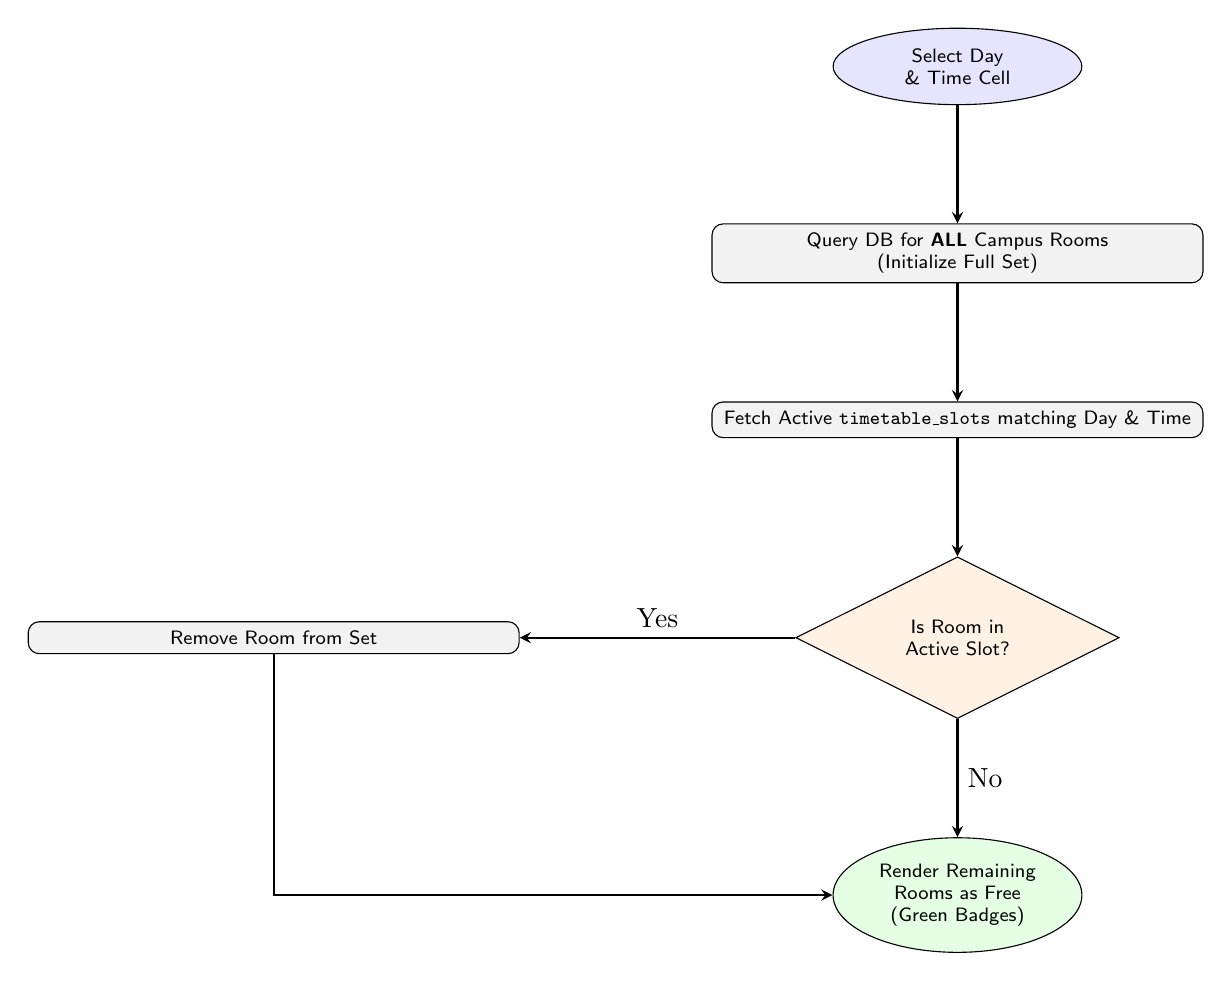
\begin{tikzpicture}[
    node distance=1.5cm,
    start/.style={draw, ellipse, fill=blue!10, text width=2cm, align=center, font=\sffamily\scriptsize},
    process/.style={draw, rectangle, fill=gray!10, text width=6cm, align=center, rounded corners, font=\sffamily\scriptsize},
    decision/.style={draw, diamond, aspect=2, fill=orange!10, text width=2.5cm, align=center, font=\sffamily\scriptsize},
    arrow/.style={draw, thick, ->, >=stealth}
]

\node[start] (init) {Select Day \& Time Cell};
\node[process, below=of init] (fetch) {Query DB for \textbf{ALL} Campus Rooms\\(Initialize Full Set)};
\node[process, below=of fetch] (active) {Fetch Active \texttt{timetable\_slots} matching Day \& Time};
\node[decision, below=of active] (check) {Is Room in\\Active Slot?};
\node[process, left=of check, xshift=-2cm] (remove) {Remove Room from Set};
\node[start, below=of check, fill=green!10] (render) {Render Remaining Rooms as Free (Green Badges)};

\draw[arrow] (init) -- (fetch);
\draw[arrow] (fetch) -- (active);
\draw[arrow] (active) -- (check);
\draw[arrow] (check) -- node[above] {Yes} (remove);
\draw[arrow] (check) -- node[right] {No} (render);
\draw[arrow] (remove) |- (render);

\end{tikzpicture}
\caption{Inverted Logic Flowchart for the Free Room Finder Algorithm}
\label{fig:free_room_flow}
\end{figure}

The algorithm executes as follows:
\begin{enumerate}
    \item The system first queries the database for \textbf{all} existing rooms.
    \item It then queries the \texttt{timetable\_slots} to retrieve all currently active sessions.
    \item For every cell in the temporal matrix (Day $\times$ Time), it instantiates the complete set of all campus rooms.
    \item It iterates through the active sessions. If a session falls within the current cell's Day and Time, that session's \texttt{room\_id} is removed from the set of available rooms.
\end{enumerate}

The remaining rooms in the set are then rendered in the UI as green badges, instantly showing users where they can find empty spaces across the campus.

\section{React Component Hierarchy}

To maintain a scalable and manageable codebase, the frontend relies on a strict component tree hierarchy. Figure~\ref{fig:component_tree} illustrates the relationship between the global layout and the localized, role-based timetable viewers.

\begin{figure}[htbp]
\centering
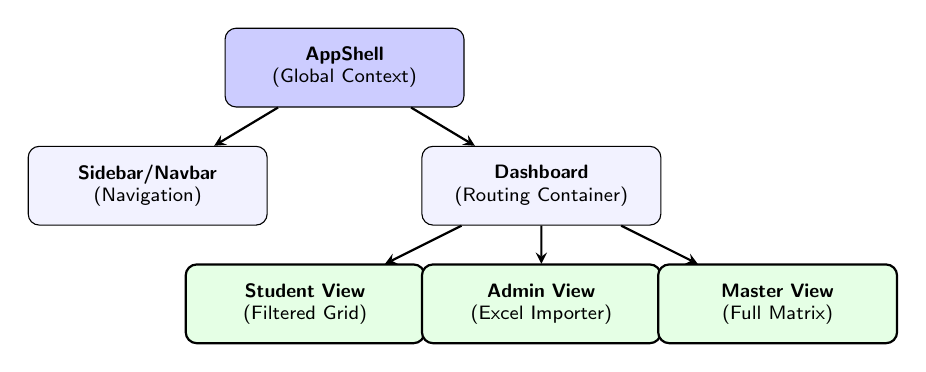
\begin{tikzpicture}[
    level 1/.style={sibling distance=5cm, level distance=1.5cm},
    level 2/.style={sibling distance=3cm, level distance=1.5cm},
    every node/.style={rectangle, draw, rounded corners, fill=blue!5, text width=2.8cm, align=center, font=\sffamily\scriptsize, minimum height=1cm},
    edge from parent/.style={draw, thick, ->, >=stealth}
]

\node[fill=blue!20] {\textbf{AppShell}\\(Global Context)}
    child {node {\textbf{Sidebar/Navbar}\\(Navigation)}}
    child {node {\textbf{Dashboard}\\(Routing Container)}
        child {node[fill=green!10] {\textbf{Student View}\\(Filtered Grid)}}
        child {node[fill=green!10] {\textbf{Admin View}\\(Excel Importer)}}
        child {node[fill=green!10] {\textbf{Master View}\\(Full Matrix)}}
    };
\end{tikzpicture}
\caption{Hierarchical Structure of the Core React Components}
\label{fig:component_tree}
\end{figure}

%-----------------------------------
\section{Role-Based Viewer Implementations}

The system provides several specialized views tailored to different stakeholders, summarized in Table~\ref{tab:view_mapping}.

\begin{table}[htbp]
\centering
\caption{Role-Based Component Mapping and Data Scope}
\label{tab:view_mapping}
\renewcommand{\arraystretch}{1.4}
\begin{tabularx}{\textwidth}{@{} l X l @{}}
\toprule
\textbf{Stakeholder Role} & \textbf{Component View} & \textbf{Primary Filter Parameter} \\
\midrule
Student & \texttt{TimetableViewer} & Semester \& Specific Section \\
Professor & \texttt{ProfessorTimetableViewer} & Faculty Email/ID \\
Department Admin & \texttt{RoomTimetableViewer} & Specific Room Name \\
Campus Admin & \texttt{MasterRoomViewer} & Building prefix (e.g., ``CC-3'', ``LT'') \\
Facility Staff & \texttt{FreeRoomViewer} & Temporal Matrix (Empty Rooms) \\
\bottomrule
\end{tabularx}
\end{table}

\subsection{Student Cohort View}
Given the complexity of modern curricula featuring numerous electives and minor tracks, a master timetable can be overwhelming. The \texttt{TimetableViewer} allows users to filter the master schedule by selecting a specific semester and section.

Crucially, it implements a \textbf{Smart Merging algorithm}. Often, core lectures are held for "All Sections" simultaneously, while practical laboratory sessions are split by specific section (e.g., "Sec A"). The merging algorithm intelligently filters the master data, pulling in slots explicitly assigned to the selected section \textit{and} slots assigned to the generic "All" section (WMC), combining them into a single, cohesive cohort schedule.

\subsection{Master Occupancy Viewer}
For campus administrators, the `MasterRoomViewer` provides a macro-level perspective. It displays a dense grid where rows represent physical rooms rather than student groups. Because an institution may have hundreds of rooms, this view implements a building-level filter. The system extracts the building prefix from the room name (e.g., identifying ``CC-3'' from ``CC-3-5106'') and allows the administrator to filter the grid, rendering a manageable overview of specific campus zones.

%-----------------------------------
\section{Export Mechanisms and Results}

To bridge the gap between the digital system and offline requirements, the platform implements robust export mechanisms.

\subsection{Client-Side PDF Generation}
Users can generate PDFs of their current view. This relies on the `html-to-image` library to capture the DOM state as a PNG, which is then embedded into a `jsPDF` document. A significant technical hurdle overcome during implementation was the handling of sticky CSS headers; the capture logic temporarily disables `position: sticky` properties on the DOM elements right before capture to ensure the entire scrollable area is rendered to the image buffer accurately.

\subsection{Google Sheets API Export}
The `RoomTimetableViewer` and `FreeRoomViewer` support bulk export directly to Google Sheets. Using the Google Identity Services client, the React application constructs a multi-layered batch update request. This request not only writes the raw string data into the cells but explicitly formats the workbookΓÇöcreating separate worksheets for different rooms, freezing header rows, applying pink and gray background colors to headers, and drawing solid bordersΓÇöresulting in a highly professional, ready-to-share document directly in the administrator's Google Drive.

\subsection{User Interface Evaluation}
The resulting application is a highly responsive, modern interface. By utilizing Tailwind CSS, the application maintains a clean, minimalist aesthetic with clear color coding (e.g., orange for practicals, green for tutorials). The elimination of page reloads between views, combined with the instantaneous clash detection, represents a monumental upgrade in usability and efficiency compared to traditional spreadsheet workflows.

%-----------------------------------
%-----------------------------------
%  NEW SECTIONS: SOLVER, EDITOR, GENERATOR
%-----------------------------------
%-----------------------------------



%-----------------------------------
\section{The Interactive Timetable Editor}
\label{sec:editor}

The \texttt{EditorView} component is where human judgment meets algorithmic output. It gives administrators an interactive, drag-and-drop interface for refining timetables---whether those timetables were generated by the solver or imported from Excel.

\subsection{Drag-and-Drop Slot Rearrangement}

The editor renders a dense 5-day $\times$ $N$-slot grid, where each scheduled session appears as a draggable card. Administrators can drag any session card from one cell to another to reassign its day and start time. The system automatically recalculates the end time based on the session's duration and validates that the new position does not fall in a lunch or break slot. All drag operations push the previous state onto a 30-level undo stack.

\subsection{Inline Editing}

Each session card exposes a hover-activated edit panel that allows inline modification of:
\begin{itemize}
    \item \textbf{Room Assignment:} A cascading two-step selector where the administrator first selects the room type (Lecture or Lab), then picks from filtered rooms of that type.
    \item \textbf{Professor Assignment:} A dropdown populated from the full professor list.
\end{itemize}

\subsection{Real-Time Conflict Visualization}

The editor implements a client-side clash detection algorithm that runs on every state change. Sessions involved in any conflict are highlighted with a red background and ring border. The algorithm checks the same constraints as the solver: room overlaps, professor overlaps, section overlaps (with elective exemptions), WMC-section conflicts, cross-basket elective clashes, and the 2+1 same-day lecture rule.

\subsection{Feasibility Check}

A dedicated ``Check Feasibility'' button constructs a full \texttt{SolverInput} from the current editor state, converts the slot positions into a \texttt{Solution} (Gene array), appends locked sessions from all other published timetables, and invokes the solver's \texttt{evaluate()} function. The result displays the total fitness score and the per-constraint violation breakdown, giving the administrator a precise understanding of remaining issues.

\subsection{LNS Auto-Fix}

When conflicts exist, the administrator can invoke the \textbf{Large Neighbourhood Search (LNS)} auto-fix~\cite{shaw1998using}. This routine:
\begin{enumerate}
    \item Identifies all session indices involved in any hard constraint violation (the ``clashing set'').
    \item Iterates for up to 1500 attempts. In each attempt, a random session from the clashing set is selected and a random mutation (relocate, time shift, or room change) is applied.
    \item If the mutation reduces the total fitness, the improved solution is accepted and the clashing set is refreshed.
    \item The process terminates early if all hard violations reach zero.
\end{enumerate}

The LNS targets only the problematic sessions rather than reoptimizing the entire schedule, making it significantly faster than a full solver run while preserving the administrator's manual adjustments to non-conflicting sessions. Figure~\ref{fig:lns_activity} illustrates this destroy-and-repair process.

\begin{figure}[htbp]
\centering
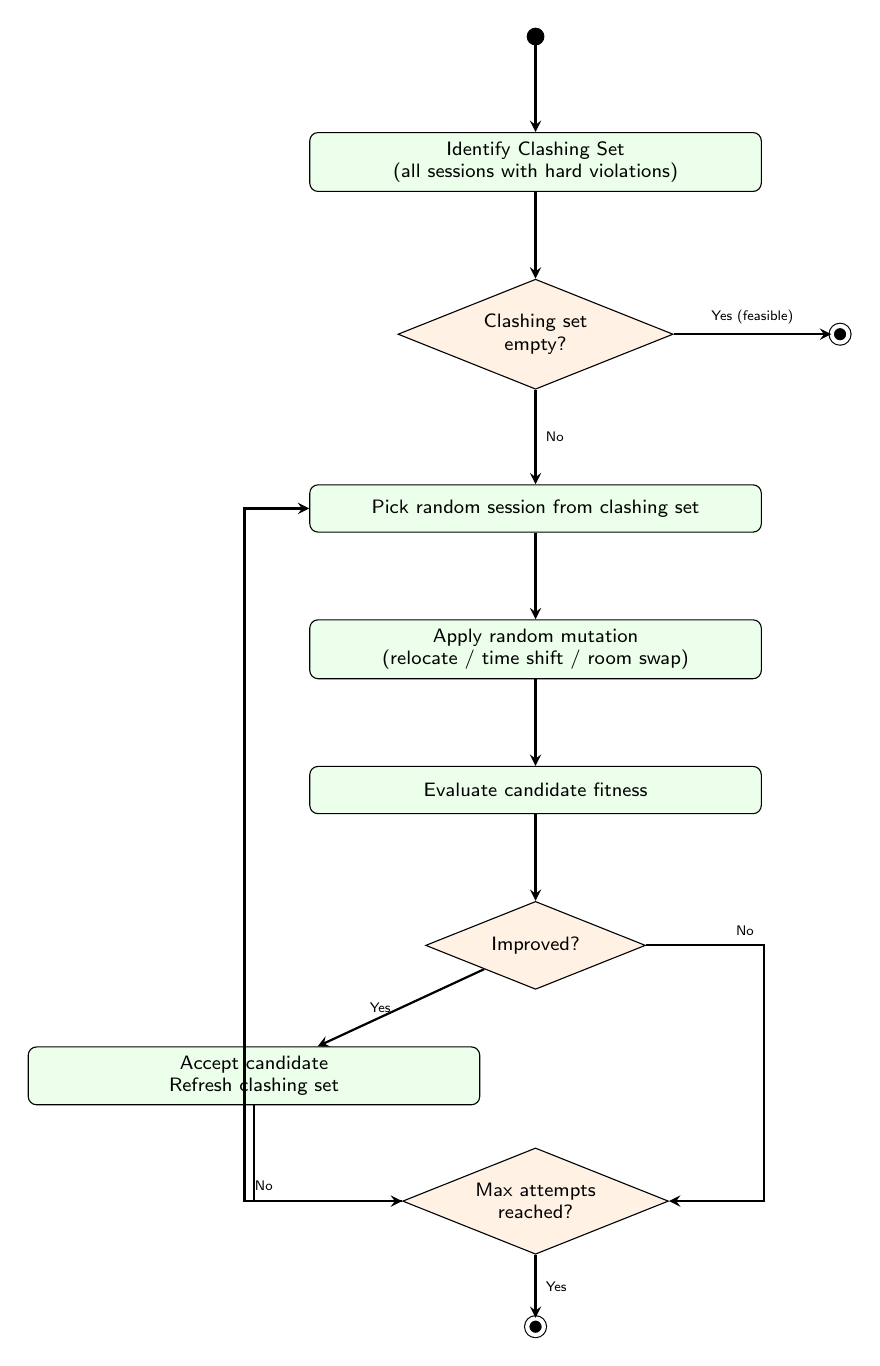
\begin{tikzpicture}[
    node distance=1.1cm,
    start/.style={draw, circle, fill=black, minimum size=6pt, inner sep=0pt},
    stop/.style={draw, circle, fill=black, minimum size=6pt, inner sep=0pt, double, double distance=1.5pt},
    action/.style={draw, rectangle, fill=green!8, rounded corners=3pt, text width=5.5cm, align=center, font=\sffamily\scriptsize, minimum height=0.6cm},
    decision/.style={draw, diamond, aspect=2.5, fill=orange!10, text width=2cm, align=center, font=\sffamily\scriptsize, inner sep=1pt},
    arrow/.style={draw, thick, ->, >=stealth, font=\sffamily\tiny}
]

\node[start] (s) {};
\node[action, below=of s] (find) {Identify Clashing Set\\(all sessions with hard violations)};
\node[decision, below=of find] (empty) {Clashing set\\empty?};
\node[action, below=1.2cm of empty] (pick) {Pick random session from clashing set};
\node[action, below=of pick] (mut) {Apply random mutation\\(relocate / time shift / room swap)};
\node[action, below=of mut] (ev) {Evaluate candidate fitness};
\node[decision, below=of ev] (better) {Improved?};
\node[action, below left=1cm and 0cm of better] (acc) {Accept candidate\\Refresh clashing set};
\node[decision, below=2cm of better] (maxiter) {Max attempts\\reached?};
\node[stop, right=2cm of empty] (done1) {};
\node[stop, below=0.8cm of maxiter] (done2) {};

\draw[arrow] (s) -- (find);
\draw[arrow] (find) -- (empty);
\draw[arrow] (empty) -- node[right] {No} (pick);
\draw[arrow] (empty) -- node[above] {Yes (feasible)} (done1);
\draw[arrow] (pick) -- (mut);
\draw[arrow] (mut) -- (ev);
\draw[arrow] (ev) -- (better);
\draw[arrow] (better) -- node[left] {Yes} (acc);
\draw[arrow] (better.east) -- ++(1.5,0) node[above left, font=\sffamily\tiny] {No} |- (maxiter);
\draw[arrow] (acc) |- (maxiter);
\draw[arrow] (maxiter) -- node[right] {Yes} (done2);
\draw[arrow] (maxiter.west) -- ++(-2,0) node[above right, font=\sffamily\tiny] {No} |- (pick);

\end{tikzpicture}
\caption{Activity Diagram: LNS Destroy-and-Repair Auto-Fix}
\label{fig:lns_activity}
\end{figure}

 
% Chapter 6

\chapter{Conclusion and Future Work} % Main chapter title

\label{Chapter6} % For referencing the chapter elsewhere, use \ref{Chapter6}

%----------------------------------------------------------------------------------------

The administration of university timetables is a complex logistical challenge that directly impacts the daily lives of students, faculty, and administrative staff. This thesis detailed the design, architecture, and implementation of the IIITA Timetabling System, a modern web-based platform built to digitize, analyze, generate, edit, and distribute academic schedules efficiently. 

%-----------------------------------
\section{Summary of Contributions}

The primary contribution of this project is the successful transition from static, error-prone spreadsheet management to a dynamic, intelligent, cloud-synchronized platform capable of both automated schedule generation and interactive refinement. 

Specific achievements include:
\begin{itemize}
    \item \textbf{Heuristic Ingestion Engine:} The development of a robust Excel parsing module capable of interpreting human-formatted spreadsheets. By utilizing heuristic rules to detect headers, extract metadata, and resolve cell merges, the system drastically reduces the friction of onboarding legacy data into a structured PostgreSQL database.
    \item \textbf{Real-Time Conflict Resolution:} The implementation of a multi-dimensional $O(N^2)$ clash detection algorithm that automatically surfaces Room, Professor, Section, and WMC-Section overlaps. This feature alone significantly reduces the administrative burden of manually verifying schedule integrity.
    \item \textbf{(1+1)-ES Automated Solver:} The implementation of a fully functional timetable generator using a (1+1) Evolution Strategy algorithm. The solver evaluates candidate schedules against a comprehensive fitness function comprising ten hard constraints (room, professor, and group non-overlap; break/lunch boundary enforcement; lab-room assignment; elective basket synchronization; WMC-section isolation; home-room binding; the 2+1 lecture format; and time boundary compliance) and three soft constraints (student schedule gaps, room utilization efficiency, and professor same-half-day avoidance). The algorithm employs Rechenberg's 1/5th success rule for adaptive step-size control and a stagnation restart mechanism.
    \item \textbf{Interactive Timetable Editor:} The development of a drag-and-drop editing interface with real-time conflict visualization, inline room and professor editing, a 30-level undo stack, and a Large Neighbourhood Search (LNS) auto-fix routine that targets clashing sessions. The editor's Master View provides cross-semester constraint awareness by overlaying slots from all published timetables.
    \item \textbf{Multi-Step Generator Wizard:} The creation of a guided configuration workflow enabling administrators to select semester clusters, auto-map home rooms using a floor-based naming policy, assign professors via an interactive matrix with expertise-based filtering, and configure seed and locked timetables before launching the solver.
    \item \textbf{Cross-Semester Constraint Awareness:} The implementation of locked sessions from published timetables, enabling the solver and editor to detect and avoid room and professor conflicts across independently scheduled semesters.
    \item \textbf{Stakeholder-Specific Interfaces:} The creation of dynamic, role-based visualization components. The personalized ``Student Custom Timetable'' with localized preference persistence, the dedicated ``Professor View,'' and the macro-level ``Master Occupancy'' and ``Free Room Finder'' views ensure that every user receives actionable data without cognitive overload.
    \item \textbf{Modern Technical Architecture:} The deployment of a high-performance frontend utilizing React 19, TypeScript, and Vite, paired with a serverless Supabase backend. This stack ensures the application is highly responsive, strictly typed, and easily maintainable.
    \item \textbf{Professional Export Capabilities:} The integration of client-side PDF generation and automated Google Sheets API formatting, bridging the gap between dynamic web views and the necessity for static, offline documentation.
\end{itemize}

%----------------------------------------------------------------------------------------
\section{Current Limitations and Proposed Enhancements}

While the current system represents a massive upgrade over traditional methods, several limitations define the boundaries of the current implementation. These limitations directly inform the proposed future work, as summarized in Table~\ref{tab:future_scope}.

\begin{table}[htbp]
\centering
\caption{System Limitations and Future Enhancements}
\label{tab:future_scope}
\renewcommand{\arraystretch}{1.5}
\begin{tabularx}{\textwidth}{@{} l X X @{}}
\toprule
\textbf{Domain} & \textbf{Current Limitation} & \textbf{Proposed Enhancement} \\
\midrule
\textbf{Data Ingestion} & Heavily reliant on hardcoded regular expressions to parse IIITA's specific Excel format. & Implementation of a dynamic mapping UI allowing users to visually map Excel columns to DB fields. \\
\textbf{Solver Performance} & Single-threaded (1+1)-ES running on the browser's main thread via batched \texttt{setTimeout}. Sufficient for current problem sizes but may become a bottleneck for larger institutions. & Migration to Web Workers for parallel solver execution, or a server-side solver for larger problem instances. Exploration of hybrid meta-heuristics (e.g., memetic algorithms combining ES with local search). \\
\textbf{Solver Optimality} & The Evolution Strategy is a meta-heuristic; solutions are feasible but not guaranteed to be globally optimal with respect to soft constraints. & Investigation of multi-objective optimization (Pareto-optimal fronts) and hybridization with constraint programming (CP) solvers for provable optimality on subproblems. \\
\textbf{State Management} & Relies on localized React state and custom hooks, potentially causing prop-drilling in deep components. & Adoption of a global state manager (e.g., Zustand or Redux) to optimize data sharing across views. \\
\textbf{Notifications} & Users must actively check the web portal for schedule updates. & Development of a Progressive Web App (PWA) with Push Notifications via Firebase Cloud Messaging. \\
\textbf{Analytics} & Basic occupancy visualization without long-term historical analysis. & Dedicated BI Dashboard to track room utilization metrics across multiple academic years. \\
\bottomrule
\end{tabularx}
\end{table}

%-----------------------------------
\section{Concluding Remarks}

In conclusion, the IIITA Timetabling System successfully modernizes a critical institutional workflow. By combining heuristic data extraction with a robust relational database, a (1+1) Evolution Strategy solver, an interactive drag-and-drop editor with LNS-based auto-fix, and a lightning-fast React frontend, the system provides unparalleled visibility, automation, and integrity to academic scheduling. The system demonstrates that a browser-based, pure-TypeScript solver can reliably generate feasible, high-quality timetables for a real-world university setting, while the interactive editor empowers administrators to refine solutions with full constraint awareness. It stands as a testament to the power of modern web technologies and evolutionary computation in solving complex, real-world logistical challenges.


\end{spacing}

%----------------------------------------------------------------------------------------
%	THESIS CONTENT - APPENDICES
%----------------------------------------------------------------------------------------

\appendix % Cue to tell LaTeX that the following "chapters" are Appendices

% Include the appendices of the thesis as separate files from the Appendices folder
% Uncomment the lines as you write the Appendices

% Appendix A

\chapter{Core Algorithm Snippets} % Main appendix title

\label{AppendixA} % For referencing this appendix elsewhere, use \ref{AppendixA}

This appendix provides crucial code excerpts from the React 19 codebase, demonstrating the practical implementation of the theoretical concepts discussed in the main chapters.

\section{Dynamic Grid Generation Logic}
The following TypeScript snippet from the \texttt{TimetableViewer} component demonstrates how the system extracts unique time boundaries to dynamically generate responsive column headers, preventing the display of empty, unused time blocks.

\begin{lstlisting}[language=java, caption={Dynamic Time Column Extraction Algorithm}]
// Extract all unique start and end times from the active slots
const allTimes = useMemo(() => {
  const times = new Set<string>();
  
  // Inject hardcoded institutional break times
  times.add("10:50");
  times.add("11:00");
  times.add("13:00");
  times.add("14:30");
  
  // Extract times from all valid timetable slots
  slots.forEach(slot => {
    if (slot.start_time && slot.end_time) {
      times.add(slot.start_time.substring(0, 5));
      times.add(slot.end_time.substring(0, 5));
    }
  });

  // Sort chronologically and format as standard columns
  return Array.from(times).sort().reduce((acc, curr, index, arr) => {
    if (index < arr.length - 1) {
      acc.push(`${curr}-${arr[index + 1]}`);
    }
    return acc;
  }, [] as string[]);
}, [slots]);
\end{lstlisting}

\section{Real-Time Clash Detection Filter}
This snippet illustrates the $O(N^2)$ comparison logic used to immediately identify Room, Professor, and Section overlaps within the currently selected semester block.

\begin{lstlisting}[language=java, caption={Overlap Detection and Categorization Logic}]
// O(N^2) comparison to find all overlapping events
const newClashes = filteredSlots.filter((slot, i) => {
  return filteredSlots.some((otherSlot, j) => {
    // Skip self-comparison
    if (i === j) return false;
    // Must be on the same day to clash
    if (slot.day_of_week !== otherSlot.day_of_week) return false;
    
    // Check for temporal intersection
    const isTimeOverlap = slot.start_time < otherSlot.end_time && 
                          slot.end_time > otherSlot.start_time;

    if (isTimeOverlap) {
      // 1. Room Clash
      if (slot.rooms?.name === otherSlot.rooms?.name) return true;
      // 2. Professor Clash
      if (slot.professors?.name === otherSlot.professors?.name) return true;
      // 3. Section Clash (Same section, different subject)
      if (slot.student_groups?.name === otherSlot.student_groups?.name &&
          slot.subjects?.id !== otherSlot.subjects?.id) {
          return true;
      }
    }
    return false;
  });
});
\end{lstlisting}

\section{Solver Fitness Evaluation Function}
The following excerpt from \texttt{constraints.ts} demonstrates the combined fitness evaluation that scores a candidate timetable against all ten hard constraints and three soft constraints.

\begin{lstlisting}[language=java, caption={Combined Fitness Evaluation (constraints.ts)}]
export function evaluate(input: SolverInput, solution: Solution): FitnessResult {
    const { sessions, rooms, numDays, config } = input;

    // Count all hard constraint violations
    const timeBoundary = countTimeBoundaryViolations(sessions, solution);
    const breakCrossing = countBreakViolations(sessions, solution);
    const roomOverlap = countRoomOverlaps(sessions, solution, rooms);
    const professorOverlap = countProfessorOverlaps(sessions, solution);
    const groupOverlap = countGroupOverlaps(sessions, solution);
    const electiveSync = countElectiveSyncViolations(sessions, solution);
    const labRoom = countLabRoomViolations(sessions, solution, rooms);
    const wmcSectionOverlap = countWMCSectionOverlaps(sessions, solution);
    const homeRoom = countHomeRoomViolations(sessions, solution);
    const twoOneLecture = countTwoOneLectureViolations(sessions, solution);

    const hardViolations = timeBoundary + breakCrossing + roomOverlap +
        professorOverlap + groupOverlap + electiveSync + labRoom +
        wmcSectionOverlap + homeRoom + twoOneLecture;

    // Compute soft constraint penalties
    const gapPenalty = computeGapPenalty(sessions, solution, numDays);
    const roomUtilizationPenalty = computeRoomUtilizationPenalty(
        sessions, solution, rooms,
        config.roomUtilizationThreshold,
        config.roomOverutilizationThreshold,
    );
    const professorSameHalfPenalty = computeProfessorSameHalfPenalty(
        sessions, solution, numDays
    );

    // Weighted composite fitness
    const total = hardViolations * config.hardPenalty
        + gapPenalty * config.gapWeight
        + roomUtilizationPenalty * config.roomUtilizationWeight
        + professorSameHalfPenalty * config.professorSameHalfWeight;

    return { total, hardViolations, gapPenalty,
        roomUtilizationPenalty, professorSameHalfPenalty,
        violationBreakdown: { timeBoundary, breakCrossing,
            roomOverlap, professorOverlap, groupOverlap,
            electiveSync, labRoom, wmcSectionOverlap,
            homeRoom, twoOneLecture },
    };
}
\end{lstlisting}

\section{(1+1)-ES Solver Main Loop}
The core optimization loop from \texttt{solver.ts}, showing elitist selection, $\sigma$-adaptation via the 1/5th success rule, and stagnation restart.

\begin{lstlisting}[language=java, caption={(1+1)-ES Main Loop (solver.ts)}]
export async function runSolver(
    input: SolverInput,
    onProgress?: (p: SolverProgress) => void,
    cancelToken?: { cancelled: boolean },
    seedSolution?: Solution,
    lockedGenes?: Gene[],
): Promise<SolverResult> {
    const { config } = input;
    let parent = seedSolution
        ? seedSolution.map(g => ({ ...g }))
        : generateInitialSolution(input);

    // Pin locked genes from published timetables
    if (lockedGenes) {
        const offset = input.sessions.length - lockedGenes.length;
        for (let i = 0; i < lockedGenes.length; i++) {
            parent[offset + i] = { ...lockedGenes[i] };
        }
    }

    let bestFitness = evaluate(input, parent);
    let bestSolution = parent.map(g => ({ ...g }));
    let sigma = config.initialSigma;
    let successes = 0;

    for (let gen = 1; gen <= config.maxGenerations; gen++) {
        if (cancelToken?.cancelled) break;

        const offspring = mutate(parent, input, sigma);
        // Re-pin locked genes (mutations must not move them)
        if (lockedGenes) { /* ... pin logic ... */ }
        const offFitness = evaluate(input, offspring);

        // Elitist selection: accept if offspring is <= parent
        if (offFitness.total <= bestFitness.total) {
            parent = offspring;
            bestFitness = offFitness;
            bestSolution = offspring.map(g => ({ ...g }));
            successes++;
        }

        // 1/5th rule sigma adaptation every W generations
        if (gen % config.adaptationWindow === 0) {
            const rate = successes / config.adaptationWindow;
            if (rate > 0.2) sigma *= config.sigmaIncrease;
            else if (rate < 0.2) sigma *= config.sigmaDecrease;
            successes = 0;
        }

        // Stagnation restart
        if (stagnationCounter > stagnationThreshold) {
            parent = generateInitialSolution(input);
            // Re-pin locked genes ...
        }

        // Early termination if feasible
        if (bestFitness.hardViolations === 0) break;
    }
    return { solution: bestSolution, fitness: bestFitness, ... };
}
\end{lstlisting}

\section{LNS Auto-Fix for the Editor}
The Large Neighbourhood Search routine from \texttt{localSearch.ts}, which identifies all clashing sessions and iteratively repairs them.

\begin{lstlisting}[language=java, caption={Full LNS Destroy-and-Repair (localSearch.ts)}]
export function runFullLNS(
    input: SolverInput,
    solution: Solution,
    maxAttempts: number = 1000,
): { solution: Solution; fitness: FitnessResult } | null {
    const baseFitness = evaluate(input, solution);
    if (baseFitness.hardViolations === 0) {
        return { solution, fitness: baseFitness };
    }

    // Find all session indices involved in violations
    let clashingIndices = findClashingIndices(input, solution);
    let targets = Array.from(clashingIndices);
    let bestSolution = solution.map(g => ({ ...g }));
    let bestFitness = baseFitness;

    for (let attempt = 0; attempt < maxAttempts; attempt++) {
        const candidate = bestSolution.map(g => ({ ...g }));
        // Pick a random clashing session
        const idx = targets[Math.floor(Math.random() * targets.length)];
        const session = input.sessions[idx];

        // Apply random mutation: relocate (50%), time shift (30%), room (20%)
        const strategy = Math.random();
        if (strategy < 0.5)
            candidate[idx] = mutateRelocate(session, input.rooms);
        else if (strategy < 0.8)
            candidate[idx] = { ...candidate[idx],
                ...mutateTime(candidate[idx], session, 3.0) };
        else
            candidate[idx] = { ...candidate[idx],
                roomIndex: mutateRoom(session, input.rooms).roomIndex };

        const candidateFitness = evaluate(input, candidate);
        if (candidateFitness.total < bestFitness.total) {
            bestSolution = candidate;
            bestFitness = candidateFitness;
            if (bestFitness.hardViolations === 0) break;
            // Refresh targets after improvement
            clashingIndices = findClashingIndices(input, bestSolution);
            targets = Array.from(clashingIndices);
        }
    }
    return bestFitness.total < baseFitness.total
        ? { solution: bestSolution, fitness: bestFitness } : null;
}
\end{lstlisting}

%\include{Appendices/AppendixB}
%\include{Appendices/AppendixC}

%----------------------------------------------------------------------------------------
%	BIBLIOGRAPHY
%----------------------------------------------------------------------------------------

\printbibliography[heading=bibintoc]

%----------------------------------------------------------------------------------------
\end{sloppypar}
\end{document}  
